\documentclass[11pt]{article}
\usepackage[margin=1in]{geometry} % Adjust margins as needed
%!TEX root = ./main_source.texx
\UseRawInputEncoding
\usepackage{hyperref}
% For authors with multiple institutions
\usepackage[affil-sl]{authblk}
% For line-numbers in my document
\usepackage{lineno}

% Redefine the cite color to your preferred color

\usepackage[utf8]{inputenc}
\usepackage[T1]{fontenc}
\usepackage{anyfontsize}
\usepackage{lipsum} % For dummy text
\usepackage{microtype} % Improved font rendering
\usepackage{titlesec} % Customize section titles
\usepackage{graphicx} % For including images
\usepackage{bm}
\usepackage{svg}
\usepackage{xcolor}
% \usepackage{ulem}
\usepackage{bbm}
\usepackage{xspace}
\usepackage{tabularx}
\usepackage{stmaryrd}
\SetSymbolFont{stmry}{bold}{U}{stmry}{m}{n}
\usepackage{bbm}
\usepackage{url}            % simple URL typesetting
\usepackage{booktabs}       % professional-quality tables
\usepackage{amsfonts}       % blackboard math symbols
\usepackage{nicefrac}       % compact symbols for 1/2, etc.
\usepackage{microtype}      % microtypography
\usepackage{amsmath,amsthm}
\usepackage{tikz}
\usepackage[most]{tcolorbox}

\usepackage{natbib}
% \bibliographystyle{dinat}
% \setcitestyle{authoryear, open={[},close={]}} %Citation-related commands

%\usepackage{amssymb}
\let\Bbbk\relax
\usepackage{newtxmath}
\usepackage{letltxmacro}
\usepackage{bm}

\usepackage{soul}
\usepackage[linesnumbered,ruled,vlined]{algorithm2e}
\usepackage[compatible]{algpseudocode} 
\usepackage{bbm}
\usepackage{svg}
\usepackage{xcolor}
\usepackage{xspace}
\usepackage{stmaryrd}
\usepackage{bbm}
\usepackage{url}            % simple URL typesetting
\usepackage{booktabs}       % professional-quality tables
\usepackage{nicefrac}       % compact symbols for 1/2, etc.
\usepackage{microtype}      % microtypography
\usepackage{letltxmacro}
\usepackage{bm}
\usepackage{caption}
\usepackage{subcaption}
\usepackage{soul}
\usepackage[linesnumbered,ruled,vlined]{algorithm2e}
\usepackage[compatible]{algpseudocode} 
% \usepackage{pgfplots}
\usepackage{doi}
\usepackage{fancyvrb,cprotect}
\usepackage{centernot}
\usepackage{fancyhdr}
\graphicspath{ {assets/} }


\definecolor{amber}{rgb}{1.0, 0.49, 0.0}
\definecolor{cadmiumgreen}{rgb}{0.0, 0.42, 0.24}
\definecolor{darkcyan}{rgb}{0.0, 0.55, 0.55}
\definecolor{darkcoral}{rgb}{0.8, 0.36, 0.27}
\definecolor{azure}{rgb}{0.0, 0.5, 1.0}
\definecolor{bittersweet}{rgb}{1.0, 0.44, 0.37}
\definecolor{razzmatazz}{rgb}{0.89, 0.15, 0.42}
\definecolor{ballblue}{rgb}{0.13, 0.67, 0.8}
\definecolor{purple}{rgb}{0.2, 0.2, 0.6}
\definecolor{egyptianblue}{rgb}{0.06, 0.2, 0.65}
\definecolor{darkslategray}{rgb}{0.0, 0.29, 0.29}
\definecolor{bananayellow}{rgb}{1.0, 0.88, 0.21}
\definecolor{blue-violet}{rgb}{0.54, 0.17, 0.89}
\definecolor{carminepink}{HTML}{EF58A0}
\definecolor{titlecolor}{RGB}{0,74,147}
\definecolor{sectioncolor}{RGB}{0,129,255}
\definecolor{subsectioncolor}{RGB}{0,129,255}
\definecolor{definitioncolor}{rgb}{0.89, 0.0, 0.13}
\usepackage{hyperref} 

\hypersetup{
    colorlinks=true,
    linkcolor=cadmiumgreen,
    citecolor=carminepink, % Set color for citation links
    urlcolor=titlecolor % Set color for URL links
}

\newcommand{\highlight}[1]{\color{razzmatazz} #1 \color{black}}
\newcommand{\ari}[1]{\textcolor{purple}{\textbf{[Ari]:} #1}}
\newcommand{\attentionC}[1]{\textcolor{orange}{\textbf{Attention Cl\'ement:}}\textcolor{blue}{\quad#1}}
\newcommand{\ykResolved}[1]{\textcolor{orange}{\textbf[YK] \sout{#1}}}
\newcommand{\CC}[1]{\textcolor{carminepink}{\textbf[CC] #1}}
\newcommand{\CCResolved}[1]{\textcolor{carminepink}{\textbf[CC] \sout{#1}}}
\usepackage{cleveref}       % smart cross-referencing


\usepackage{framed}
\usepackage{rotating}

\usepackage[colorinlistoftodos]{todonotes}
% todo leftbar
% \newenvironment{todo}{ %
% \def\FrameCommand{\hspace{-2em}%
% \begin{sideways}%
% \textcolor{red}{\textsf{\small TODO}}%
% \end{sideways}%
% \hspace{0.5em}\textcolor{red}{\vrule width 0.5pt} \hspace{0.5em}}\MakeFramed {\advance\hsize-\width \FrameRestore}}
% {\endMakeFramed}



%\newcommand{\email}[1]{\texttt{#1}}
\usepackage{accents}
\usepackage{calc}
%%%%%%%%%%%%%%%%%%%%%%%%%%%%%%
% Theorem
% Define a new theorem style
\newtheoremstyle{theoremstyle}
  {\topsep} % Space above
  {\topsep} % Space below
  {} % Body font
  {} % Indent amount
  {\bfseries\color{black}} % Theorem head font
  {} % Punctuation after theorem head
  {.5em} % Space after theorem head
  {\thmname{#1}~\thmnumber{#2}:~\textcolor{carminepink}{\thmnote{[#3]}}} % Theorem head spec (can be left empty, meaning ‘normal’)

% Define mdframed settings for the lemma box
\mdfdefinestyle{theoremframe}{
  linecolor=theoremcolor!80,
  linewidth=2pt,
  backgroundcolor=theoremcolor!15,
  roundcorner=5pt,
  nobreak=true,
  topline=false,
  bottomline=false,
  rightline=false,
}
% Apply the custom theorem style
\theoremstyle{theoremstyle}
% Define a theorem environment
\newtheorem{theorem}{Theorem}[section]
% Automatically surround lemma with mdframed
\surroundwithmdframed[style=theoremframe]{theorem}


%%%%%%%%%%%%%%%%%%%%%%%%%%%%%%
% Remark
\newtheoremstyle{remarkstyle}
  {\topsep} % Space above
  {\topsep} % Space below
  {} % Body font
  {} % Indent amount
  {\bfseries\color{black}} % Theorem head font
  {} % Punctuation after theorem head
  {0.5em} % Space after theorem head
  {} % Theorem head spec (can be left empty, meaning ‘normal’)

% Define mdframed settings for the lemma box
\mdfdefinestyle{remarkframe}{
  linecolor=fuyu-gaki!80,
  linewidth=2pt,
  backgroundcolor=fuyu-gaki!15,
  roundcorner=5pt,
  nobreak=true,
  topline=false,
  bottomline=false,
  rightline=false,
}
% Apply the custom theorem style
\theoremstyle{remarkstyle}
\newtheorem{remark}{Remark}
\surroundwithmdframed[style=remarkframe]{remark}
\newtheorem{corollary}{Corollary}
\surroundwithmdframed[style=remarkframe]{corollary}

\newtheoremstyle{definitionstyle}
  {\topsep} % Space above
  {\topsep} % Space below
  {} % Body font
  {} % Indent amount
  {\bfseries\color{black}} % Theorem head font
  {} % Punctuation after theorem head
  {.5em} % Space after theorem head
  {\thmname{#1}~\thmnumber{#2}:~\textcolor{carminepink}{\thmnote{[#3]}}} % Theorem head spec (can be left empty, meaning ‘normal’)

% Define mdframed settings for the lemma box
\mdfdefinestyle{definitionframe}{
  linecolor=definitioncolor!80,
  linewidth=2pt,
  backgroundcolor=definitioncolor!45,
  roundcorner=5pt,
  nobreak=true,
  topline=false,
  bottomline=false,
  rightline=false,
}
\theoremstyle{definitionstyle}
\newtheorem{definition}[theorem]{Definition}
\surroundwithmdframed[style=definitionframe]{definition}

%%%%%%%%%%%%%%%%%%%%%%%%%%%%%%
% Lemma
% Define a new theorem style
\newtheoremstyle{lemmastyle}
  {\topsep} % Space above
  {\topsep} % Space below
  {} % Body font
  {} % Indent amount
  {\bfseries\color{black}} % Theorem head font
  {} % Punctuation after theorem head
  {.5em} % Space after theorem head
  {\thmname{#1}~\thmnumber{#2}:~\textcolor{carminepink}{\thmnote{[#3]}}} % Theorem head spec (can be left empty, meaning ‘normal’)

% Define mdframed settings for the lemma box
\mdfdefinestyle{lemmaframe}{
  linecolor=theoremcolor!80,
  linewidth=2pt,
  backgroundcolor=theoremcolor!05,
  roundcorner=5pt,
  nobreak=true,
  topline=false,
  bottomline=false,
  rightline=false,
}
% Apply the custom theorem style
\theoremstyle{lemmastyle}
\newtheorem{lemma}[theorem]{Lemma}
% Automatically surround lemma with mdframed
\surroundwithmdframed[style=lemmaframe]{lemma}
\newtheorem{claim}[theorem]{Claim}
% Automatically surround lemma with mdframed
\surroundwithmdframed[style=definitionframe]{claim}

% Define custom environments for Question and Open Problem
% \newenvironment{question}
%   {\reversemarginpar
%    \marginnote{\textbf{\textcolor{fuyu-gaki}{Question:}}}}
%  {}

\newtcolorbox[auto counter, number within=section]{problem}[2][]{colframe=fuyu-gaki, colback=mizu!10, coltitle=white, title={Problem }, sharp corners, boxrule=0.8mm, width=0.99\textwidth, boxsep=2mm, left=3mm, right=3mm, top=2mm, bottom=2mm, breakable}



%%%%%%%%%%%%%%%%%%%%%%%%%%%%%%
\newcommand{\goal}[1]{
\begin{tcolorbox}[colframe=red!50!black, colback=white!95!black,title=Goal]
#1
\end{tcolorbox}    
}


% Common stuff that show up in nearly all writeups
\newcommand{\Def}{=}
\makeatletter
\newcommand{\smalldollar}{\mathrel{\mathpalette\small@dollar\relax}}
\newcommand{\small@dollar}[2]{%
  \vcenter{\hbox{%
    $#1\textnormal{\fontsize{0.7\dimexpr\f@size pt}{0}\selectfont\$}$%
  }}%
}
\makeatother
\renewcommand{\emph}[1]{\textit{#1}}
\newcommand\Bigger[2][7]{\left#2\rule{0mm}{#1truemm}\right.}
\renewcommand{\vec}[1]{\mathbf{#1}}
\newcommand{\TODO}{\textcolor{orange}{??TODO??}}
\renewcommand{\epsilon}{\varepsilon}
\newcommand{\Set}[1]{\left\{ #1\right\}}
\newcommand{\RCloseLOpenInterval}[2]{}
\newcommand{\LCloseROpenInterval}[2]{\left[#1, #2\right)}
\newcommand{\Interval}[2]{\left[\right]}
\newcommand{\OpenInterval}[2]{\left(\right)}
\newcommand{\DistSet}[1]{\Delta(#1)}
\newcommand{\Dist}{\mathcal{D}}
\newcommand{\leftarrowS}{\leftarrow\joinrel\smalldollar}
\newcommand{\rightarrowS}{\smalldollar\joinrel\rightarrow}
\newcommand{\samples}{\highlight{\leftarrowS}}
\newcommand{\negl}{\mathtt{negl}}
\newcommand{\Indicator}[1]{\mathbbm{1}\left\{#1\right\}}
\newcommand{\Eps}{\textcolor{red}{\varepsilon}}
\newcommand{\EpsLower}{\textcolor{shin-kai}{\varepsilon'}}
\newcommand{\EpsUpper}{\textcolor{shin-kai}{\varepsilon}}
\renewcommand{\tilde}[1]{\widetilde{#1}}
\newcommand{\bit}{\{0,1\}}
\newcommand{\poly}{\mathsf{poly}}
\newcommand{\Naturals}{\mathbb{N}}
\newcommand{\Integers}{\mathbb{Z}}
\newcommand{\Reals}{\mathbb{R}}
\newcommand{\Field}{\mathbb{F}}
\newcommand{\BigO}[1]{O\left(#1\right)}
\newcommand{\BigOTilde}[1]{\tilde{O}\left(#1\right)}
\newcommand{\SmallO}[1]{o\left(#1\right)}
\newcommand{\BigOmega}[1]{\Omega\left(#1\right)}
\newcommand{\SmallOmega}[1]{\omega\left(#1\right)}
\newcommand{\Mean}[2]{\mathbb{E}_{#1}\left[#2\right]}
\newcommand{\Prob}[1]{\Pr\left[#1 \right]}
\newcommand{\PProb}[2]{\Pr_{#2}\left[#1 \right]}
\newcommand{\True}{\texttt{True}}
\newcommand{\False}{\texttt{False}}


% Complexity classes 
\newcommand{\BPP}{\mathsf{BPP}}
\renewcommand{\P}{\mathsf{P}}
\newcommand{\NP}{\mathsf{NP}}
\newcommand{\CoNP}{\mathsf{coNP}}

% Paper specific + Proof Complexity Macros
\newcommand{\PropFormula}{\Phi}
\newcommand{\Proof}{\pi}
\newcommand{\Size}[1]{|#1|}
\newcommand{\Card}[1]{\text{Card}(#1)}
\newcommand{\Axioms}{\mathcal{Q}}
\newcommand{\axiom}{q}
\newcommand{\PM}[1]{\text{PM}(#1)}
\newcommand{\RemGraph}{G'}
\newcommand{\BadSet}{\textcolor{blue}{\hat{S}}}
\newcommand{\ari}[1]{\textcolor{kon-peki}{Ari: }#1}
\newcommand{\highlight}[1]{\textcolor{yama-budo}{#1}}
\newcommand{\red}[1]{\textcolor{fuyu-gaki}{#1}}
\newcommand{\green}[1]{\textcolor{shin-ryoku}{#1}}
\newcommand{\RedNodes}[1]{\red{\text{Red}}(#1)}
\newcommand{\GreenNodes}[1]{\green{\text{Green}}(#1)}
\newcommand{\GreenB}{\green{B}}
\newcommand{\RedA}{\red{A}}
\newcommand{\BipartiteG}{G_{\GreenB \cup \GreenB}}
\newcommand{\SizeRemGraph}{n'}

% Graph Commands
\newcommand{\Graph}{G}
\newcommand{\Vertices}[1]{\mathsf{V}(#1)}
\newcommand{\Edges}[1]{\mathsf{E}(#1)}
\newcommand{\CutEdges}[3]{e(#1 \leftrightarrow #2; #3)}
\newcommand{\IncidentEdges}[1]{\mathsf{E}(\rightarrow #1)}
\newcommand{\CutEdgesSet}[3]{\mathsf{E}(#1 \leftrightarrow #2; #3)}
\newcommand{\OddComponents}[1]{q(#1)}
\newcommand{\degree}[2]{\mathsf{deg}_{#1}(#2)} 
\newcommand{\MaxDegree}[1]{\Delta_{#1}}
\newcommand{\Neighbourhood}[2]{\Gamma_{#1}\left(#2\right)}
\newcommand{\Family}[1]{\textcolor{purple}{\mathcal{#1}}}
\newcommand{\SafeStates}{\Family{S}}
\newcommand{\HardInstance}{H}
\newcommand{\Embedding}[1]{\Psi\left(#1\right)}
\newcommand{\Path}[2]{\mathsf{P}_{#1 \rightsquigarrow #2
}}
\newcommand{\PathSize}{\textcolor{red}{l}}
\newcommand{\GlobalEdgeSet}{\textcolor{orange}{\mathcal{E}}}
\newcommand{\Degree}[1]{\text{Deg}\left(#1\right)}
\newcommand{\PerfectMatching}[1]{\mathsf{PM}\left(#1\right)}
\newcommand{\Complement}[1]{\overline{#1}}
\newcommand{\EdgeConnectivity}[1]{\kappa'(#1)}
\newcommand{\PC}{\vdash_{\texttt{PC}_F}}
\newcommand{\SOS}{\vdash_{\texttt{SOS}}}
\newcommand{\en}{\textcolor{ballblue}{n}}
\newcommand{\dee}{\textcolor{cadmiumgreen}{d}}
\newcommand{\eigen}{\textcolor{red}{\lambda}}
\newcommand{\EnDeeLambda}{(n, d, \lambda)}
\newcommand{\Subdivision}[2]{{#1}^{#2}}
\newcommand{\MinimalDegree}[1]{\delta_{#1}}
\newcommand{\dbtilde}[1]{\tilde{\raisebox{0pt}[0.85\height]{$\tilde{#1}$}}}
\newcommand{\na}{\green{n_B}}
\newcommand{\EdgesShort}{E}
\newcommand{\ExpansionFactor}[1]{\lambda(#1)}
\newcommand{\EmbeddingFunc}{\Psi}



 %These are generic commands (Might move them to %base template)is


\synctex=1
% Title
\title{Sum of Squares Refutations of Perfect Matchings In Expander Graphs Is Hard}

% \author{}
\author[1]{Ari Biswas}
\author[2]{Rajko Nenadov}
\affil[1]{\small University Of Warwick, United Kingdom}
\affil[2]{\small University Of Auckland, New Zealand}

\date{}
% \linenumbers
\begin{document}

\maketitle
\begin{abstract}
This work studies the complexity of refuting the existence of a perfect matching in expander graphs with an odd number of vertices in the Sum of Squares (SoS) proof system.
In previous work, \citet{Austrin_2022} showed  SoS refutations of perfect matchings in sparse $d$-regular random graphs requires proofs with degree $\BigOmega{n/\log n}$ \highlight{on average}.
Although a $d$-regular random graph is an expander graph with high probability, their hardness result relies critically on the randomness of sampling a graph. 
Therefore, these techniques do not extend to instances where the expander graph is deterministically constructed, and thus they are unable to provide \highlight{worst-case} lower bounds.
In this work, we bridge this gap by showing SoS refutations of perfect matchings in any expander graph with a very mild spectral gap requires proofs with degree $\BigOmega{n/\log n}$.

\end{abstract}

\section{Introduction}


\begin{figure}
	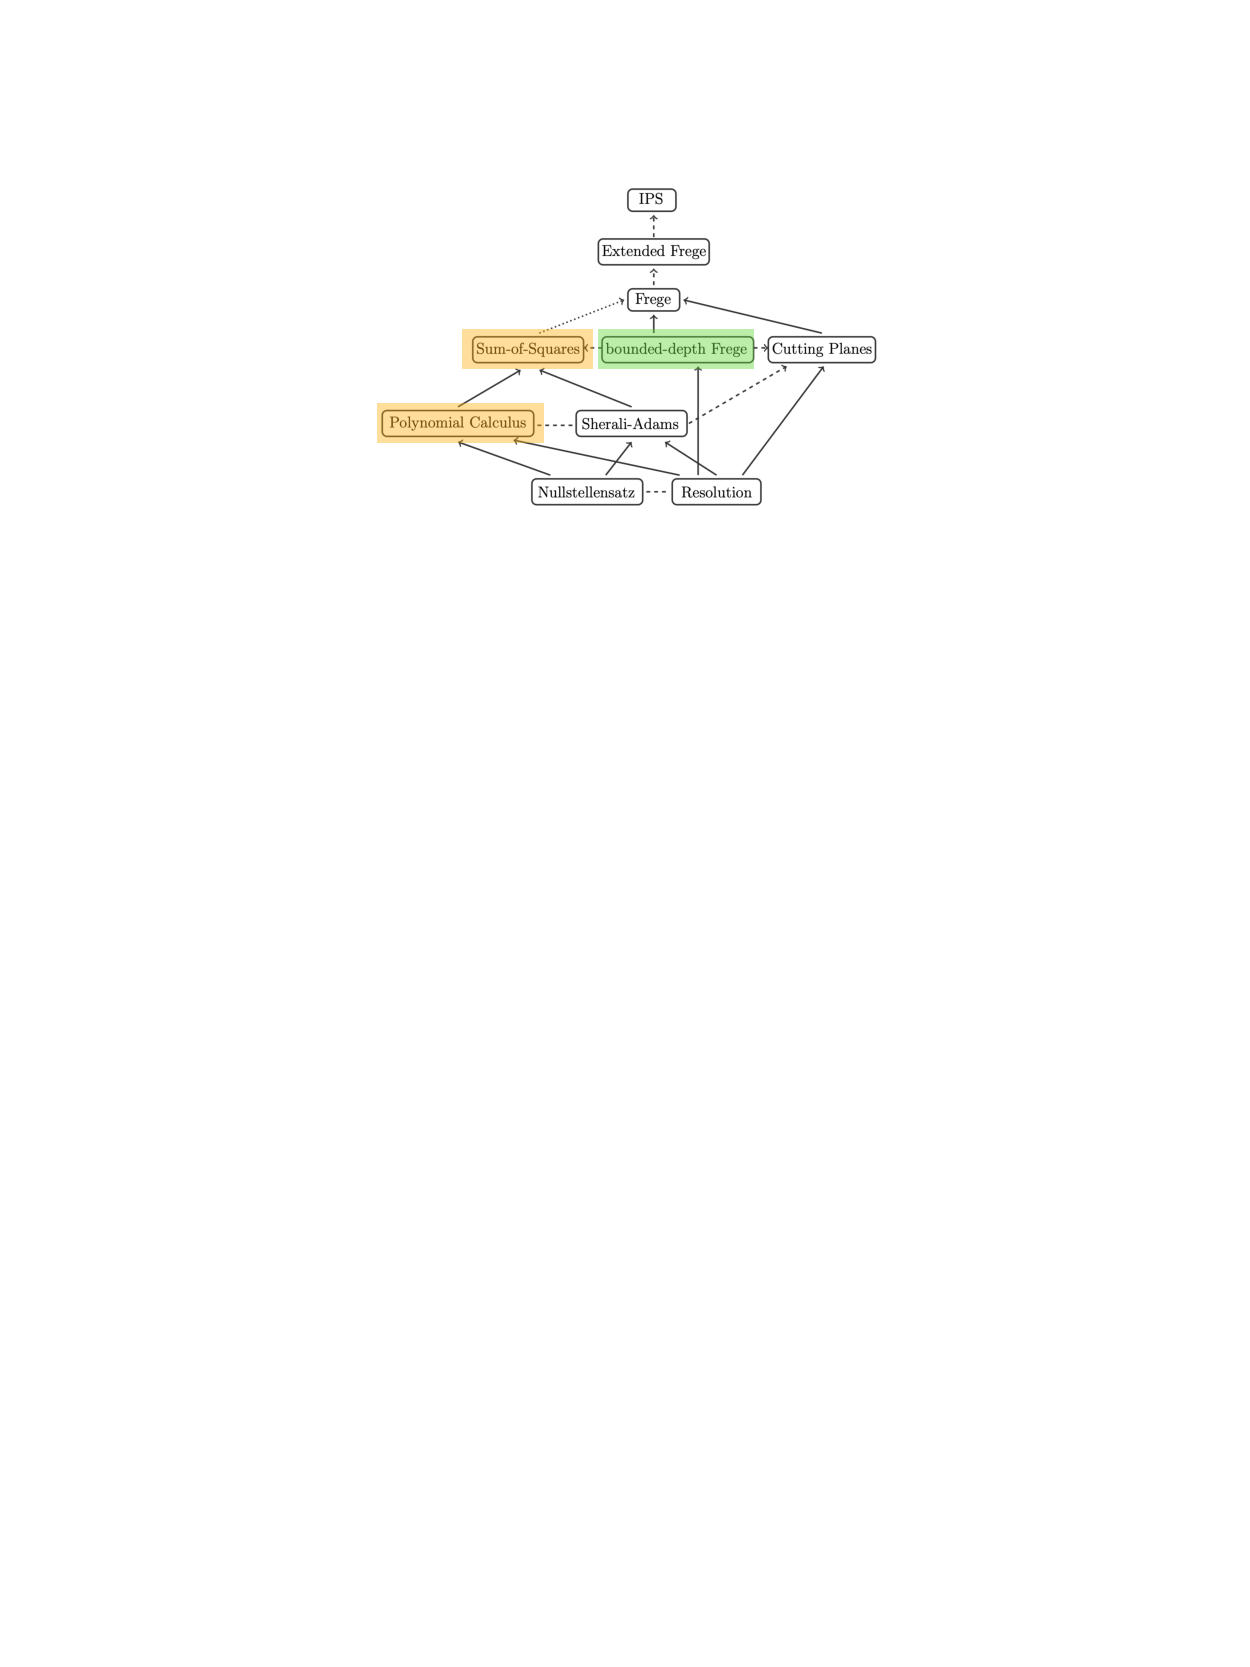
\includegraphics{assets/proof-system-relationships.pdf}
	\caption{The figure above (sourced from \citep[Page 9]{fleming2019semialgebraic}) depicts proof systems commonly studied by the community and how they relate to each other. We show lower bounds in the proof systems highlighted in orange, and as a consequence this also implies lower bounds in the bounded-depth Frege proof systems. \highlight{Change this}.}
	\label{fig:example-proof-systems}
\end{figure}


Perhaps the most fundamental problem in computation is to provide an answer to the question: ``\textit{Given a true statement $A$, is there a short proof of the claim that $A$ is true?}''
In trying to answer this question, \citet{cook1979relative} observed that we must first describe what constitutes a valid proof?
That is, we must describe the language in which the proof is written, and the rules for checking it.
Each set of rules for writing and checking a proof defines a proof system.
Therefore, a precise restatement of the question above is the following:  ``\textit{Given a true statement $A$ and a proof system $S$, what is the length of the shortest proof $\Proof \in S$ that proves $A$?}''
If we could show that there exists a proof system $S$, such that for any true statement $A$, the length of the shortest proof in $S$ is upper bounded by some polynomial in the length of $A$, it would imply that $\CoNP = \NP$, which would further imply that $\P = \NP$.
Conversely, if we could show large proof size lower bounds for $A$ in \emph{all} proof systems, it would lead to a formal proof of the widely believed conjecture that $\P \neq \NP$.
Unfortunately, we currently do not possess the tools to show lower such bounds for \emph{arbitrary} proof systems.
Thus, as an intermediate step towards making partial progress towards the grand problem, the research community has invested a significant amount of time and energy in proving size lower bounds for certain specific proof systems \citep{blake1937canonical,razborov1998lower, impagliazzo1999lower, alekhnovich2001lower, buss1999linear}.
 Figure \ref{fig:example-proof-systems} lists some these proof systems and describes the relationships between them.
Proof systems listed at the top of Figure \ref{fig:example-proof-systems} are more expressive\footnote{Expressiveness is formalised by the notion of $p$-simulation, and we refer the reader to \citep[Definition 1.6]{ProofComplexityLecNotes} for more details.}, and lower bounds for such proof systems subsume claims about the complexity of proofs lower in the figure.
We refer the reader to \citep{krajicek2019proof, ProofComplexityLecNotesPaul} for more details on the definitions of the various proof systems.
In this work, we focus on the semi-algebraic proof system of sum of squares (SoS) \citep{parrilo2000structured, boazCourse}.
In proof systems like SoS, instead of a propositional formula over $n$ variables, we are given a set $\Axioms =\{\axiom_i(\vec{x}) \text{ } |\text{ } i \in [m] \}$ of $m$ polynomial equations\footnote{Semi-algebraic proof systems also allow for inequalities but we will not deal with inequality constraints in this paper.} over $n$ variables $\vec{x} = \{x_1, \dots, x_n\}$ with real coefficients as the problem instance.
We say a proof $\Proof$ is a refutation of $\Axioms$, if it is a proof of the claim (in the specified language) that there exists no assignment of $\vec{x} \in \Field^n$ that satisfies \emph{all} the polynomial equations in $\Axioms$. 
In SoS, the proof $\Proof$ is itself expressed as a sequence of polynomials, and the size/complexity of the proof is measured by the degree of the proof polynomials that refutes $Q$ (see Section \ref{sec:proof-system-prelims} for more formal details).
We denote the minimum degree over all proofs that refute $\Axioms$ with $\Degree{Q \SOS \bot}$, and the main goal of the area is to study how large is the degree of proofs for refuting a given set of axioms $\Axioms$.
Another important reason for proving lower bounds for algebraic proof systems is that these can be used to then get lower bounds for a broad family of related algorithms \highlight{cite}.
Similarly, proof system upper bounds has led to the fruitful discovery of many efficient algorithms \highlight{cite}.
The SoS proof system is of particular interest because of its close connection to the sum-of-squares hierararchy of semi-definite programming.
We refer the reader to \citep[Chapter 3]{fleming2019semialgebraic} for more details.
In this paper we consider refutations of the \emph{perfect matching principle}.
Apart from being a natural well studied problemn in its own right, the perfect matching principle is also related to the widely studied pigeon hole principle (PGP) \citep{razbarov2002pgp} and Tseitin formula \citep{grigoriev2001linear}.
Assuming at most one pigeon fits in a single hole, the pigeon hole principle says $m$ pigeons cannot fit in $n < m$ holes.
If we construct a bipartite graph with the left vertices as $m$ pigeons and the right vertices as $n$ holes, proving the pigeon hole principle amounts to proving the graph does not have a perfect matching.
There are many variants of the pigeon hole principle (see \citep{razbarov2002pgp}), and almost all of them are easy to refute in the sum of squares proof system.
The Tseitin formula over a graph claims that there is a subgraph for which every vertex has odd degree.
If a graph has a perfect matching, then the subgraph described by the matching ensures that every vertex has odd degree.
For graphs on an odd number of vertices this is clearly impossible.
However, formally refuting this claim for expandeer graphs in the SoS proof system, requires size linear in the number of vertices in the graph \cite{grigoriev2001linear}.
Given its close connections to refuations of the PGP and Tseitin principle, it is natural to study the complexity of refuting perfect matchings for non-bipartite graphs in greater detail.
It is conjectured that complexity of refuting perfect matchings is in between Tseitin and PGP.\par
Matchings are a combinatorial concept. To refute matchings with an algebraic proof system, we need to find a way to express the combinatorial constraints as algebraic inequalities.
More specifically, given an undirected graph $G=(V,E)$, and a vector $\vec{b} = (b_1, \dots, b_{|V|})  \in \Field^{\Size{V}}$, we define $\Card{G, \vec{b}}$ as the following set of polynomial constraints over variables $x_1, \dots, x_{|E|} \in \Field^{\Size{E}}$

\[
        \Card{G, \vec{b}}=
        \Bigger[10]\{\begin{array}{@{}cl}
                x_{\highlight{e}}(1 - x_{\highlight{e}}) = 0 & \text{ for every $\highlight{e} \in E$}\\[3mm]
                \underset{u \text{ is a neighbour of }\highlight{v}}{\sum x_{(u,\highlight{v})}}= b_{\highlight{v}} & \text{ for every $\highlight{v} \in V$} \\[3mm]
        \end{array}
\]

For every $e \in E$, if the polynomial equation $x_e(1 - x_e) = 0$ were to be satisfied, then it restricts the domain of the above variables to bits i.e. $x_e \in \bit$ for all $e \in E$.
Note if there was an assignment of variables in $\vec{x} \in \bit^{|E|}$ that satisfied all the equations in $\Card{G, 1^{|V|}}$, it would imply that the graph $G$ has a perfect matching (given by the edges corresponding to variables with assignment 1).  
When $\vec{b} = 1^{|V|}$, as short hand we denote $\Card{G, \vec{b}}$ as $\PM{G}$.
When $|V|$ is odd, we know that any graph $G$ cannot have a perfect matching.
In other words, $\Card{G, 1^{|V|}}$ cannot be satisfied.
In this work we are interested in the complexity refutations for $\PM{G}$  when $|V|$ is odd in PC and SoS proof systems.
With no further constraints on $G$, generic lower bounds for these refutations in PC or SOS proof systems are not known.
In recent work \citet{Austrin_2022} made progress in proving lower bounds by showing that refuting the existence of perfect matchings in \emph{random $d$-regular graphs} in the Sum-of-Squares and Polynomial Calculus proof system requires long proofs.
More formally, they show that 

\begin{theorem}\label{thm:prev-thm}
There is a constant $d_0 \in \Naturals$ such that for all $d \geq d_0$, the following holds \emph{asymptotically almost surely} over a random $d$-regular graph $G=(V,E)$ on $n$ vertices (where $n$ is odd)
\begin{enumerate}
    \item{ $\Degree{\Card{G, \vec{1}} \PC \bot} = \BigOmega{\frac{n}{\log n}}$} 
    \item{$\Degree{\Card{G, \vec{1}} \SOS \bot} = \BigOmega{\frac{n}{\log n}}$}
\end{enumerate}
\end{theorem}

Although random $d$ regular graphs are expander graphs with high probability, their lower bound techniques rely strongly on the randomness of sampling, and thus they are unable to extend their results to general expander graphs.
They conjecture (see \citep[Section 6]{Austrin_2022}) that the hardness results should also apply to general expander graphs, and leave showing this as an open problem. In this work, we extend their results to all expander graphs\footnote{More specifically we mean any expander graph with a very mild spectral gap $\lambda \leq \epsilonL d$ where $\epsilonL$ is a small universal constant.}, and provide worst case size lower bounds instead of average case lower bounds.

\begin{problem}

Do refutations for $\Card{G, \vec{1}}$ for
PC over fields of characteristic $\neq 2$ and SoS have large size, when $G$ is an expander graph?

\end{problem}

\begin{figure}
  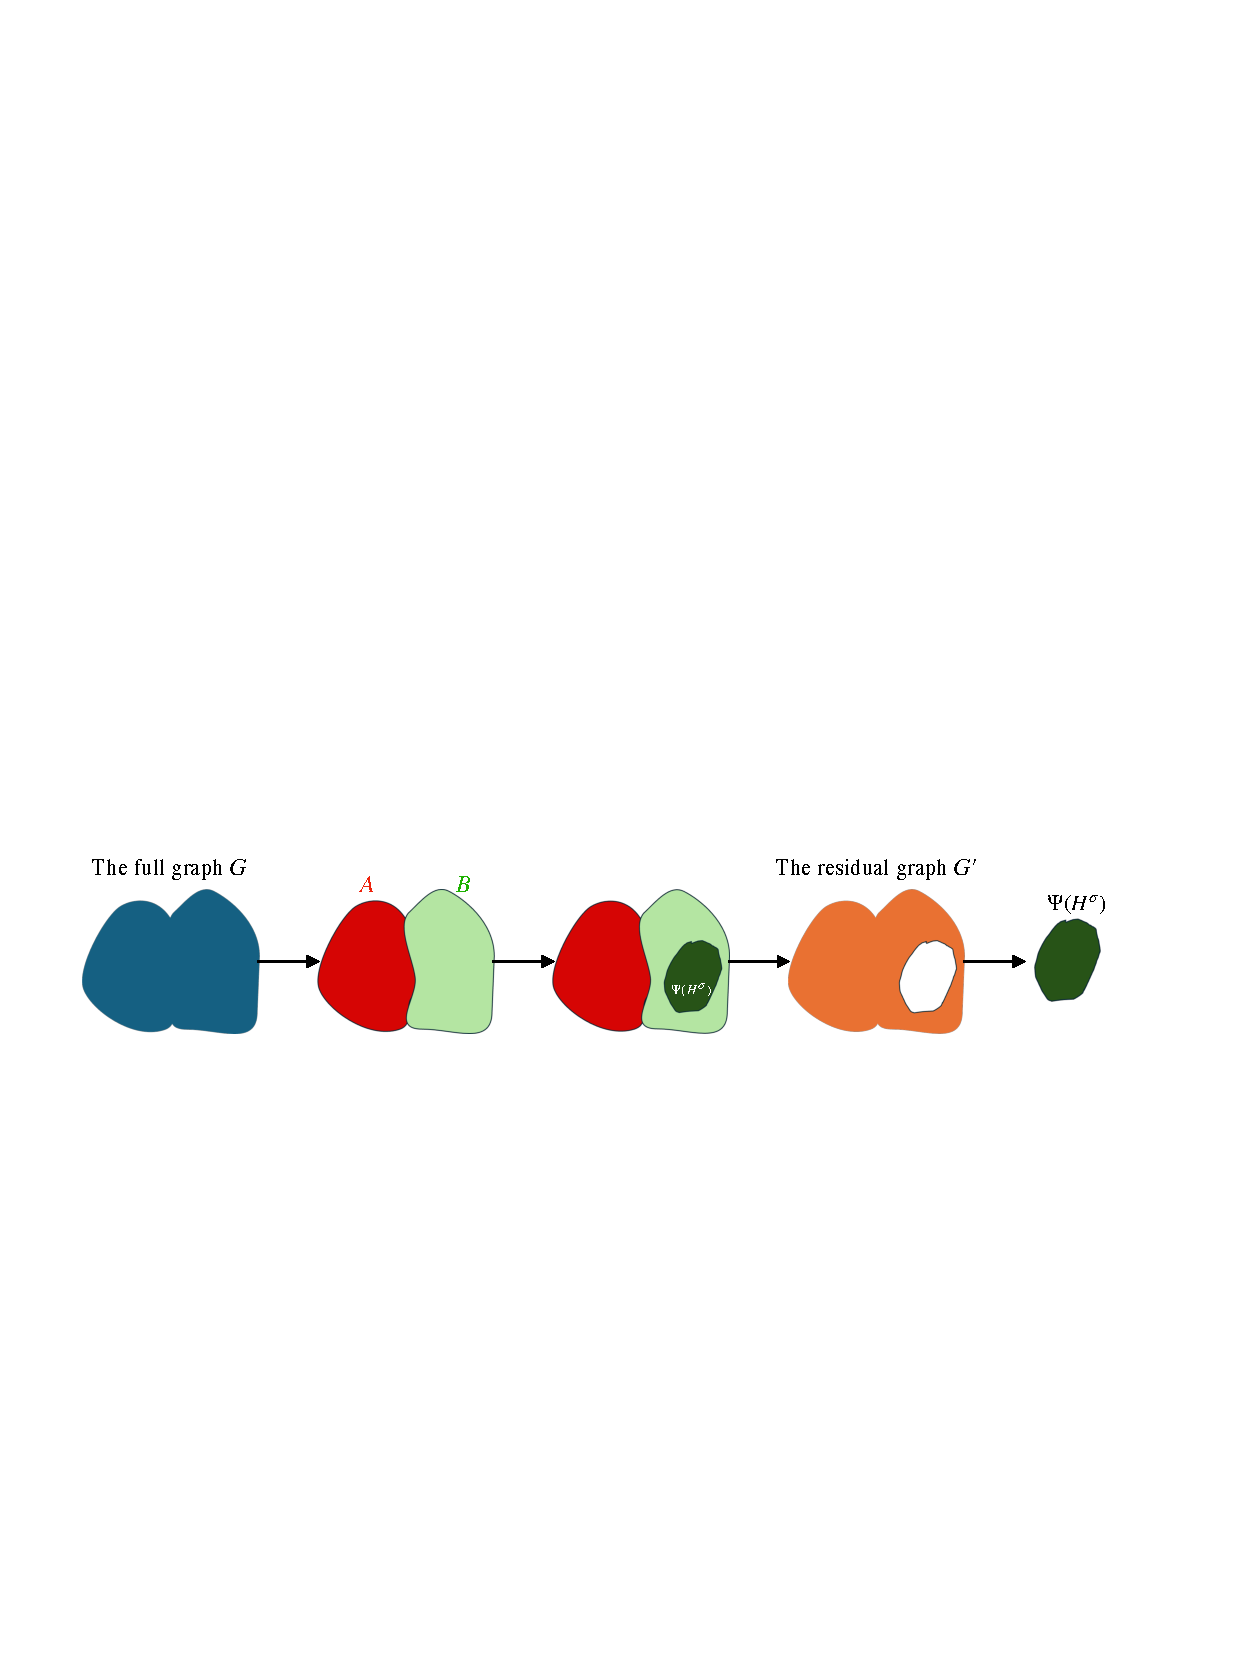
\includegraphics[width=0.8\textwidth]{assets/proof-sketch.pdf}
  \caption{The figure above above outlines the steps of the proof. First we partition the vertices of $G$ into balanced sets $\RedA$ and $\GreenB$. After that, we topologically embed the hard instance $H$ such that every path representing an edge of $e$ in the embedding is of odd size. This ensures that the graph restricted to the embedding is hard to refute. Next we show that the induced subgraph (referred to as the residual graph $\RemGraph = G[V \setminus \Embedding{\Subdivision{H}{\sigma}}]$) has a perfect matching. This  implies that the hardness to refute matchings in $G$ is transferred to the hardness of refuting $H$.} 
	\label{fig:proof-outline}
\end{figure}


\paragraph{Technical Overview} The original hardness proof works as follows.
They start with a graph $H$ on $t = \BigO{n/\log n}$ described by \citet{buss1999linear} which is known to be hard to refute (Lemma \ref{lemma:worst-case-instance-sos}).
Given a random $d$-regular graph $G\samples \mathcal{G}(n, d)$ on $n$ vertices (where $n$ is odd), the authors embed the worst case hard graph $H$ in $G$ in a way that transfers the hardness of $H$ into $G$.
A random graph is an expander graph with high probability, and there is a long line of research about embedding arbitrary graphs into expander graphs \citep{krivelevich2019completeminorsgraphssparse, kleinberg1996short}.
However to transfer hardness, it does not suffice to just embed $H$ into $G$, but we need a topological embedding of $H$ such that the parities of all the paths are the same (all paths must be of odd length).
Thus, their main technical contribution is a embedding theorem that allows for  topological embeddings of any graph $H$ into an expander graph.
To do this, they first partition the graph into two roughly equal sized sets $S$ and $T$ with sufficiently many edges in the cut between them.
Then they require that the induced subgraph $G[T]$ contains a constant degree $\alpha$ vertex expander such that the maximal degree of $H$ is $\MaxDegree{H} \ll \alpha^2 \degree{}{G}$.
The reason the authors require the second property, is to be able to extend result by \citet{krivelevich2019completeminorsgraphssparse}, which allows us to embed any graph $H$ into a host graph $\tilde{G}$ as an ordinary minor, if $\tilde{G}$ is a vertex expander with the above properties.
Now to go from minor to topological minor, a key step in their construction is that they require that the induced subgraph $G[T]$ also be odd cycle robust (see \citep[Definition 3.2]{Austrin_2022}).
To show that $G$ is odd cycle robust, their proof needs $G$ to be a random sample, as this allows them to show that the number of $i$-cycles in the graph, denoted in their paper by $Y_i(G)$ is a Poisson random variable.
Then using the tail bounds of the Poisson distribution they get what they are after with high probability.
Thus, a distinctive feature of their result is that as their embedding relies on randomness used to sample the regular graph, and they can only provide average case lower bounds.
These techniques do not apply when the host graph $G$ is constructed deterministically, as in the case of the many known deterministic constructions of expander graphs.\par

Note that just topologically embedding $H$ into $G$ is still not sufficient to show that perfect matchings in $G$ are hard to refute.
It is entirely possible that the residual graph which does not contain an embedding of $H$ has evidence that allows us to refute the existence of a perfect matching with shorter proofs (for example it may have an isolated vertex).
One way to prevent this possibility is to show that the residual graph has a perfect matching.
As $n$ is odd, this could mean that the hardness of refuting perfect matchings \emph{must} come from the embedding only.
To show that the residual graph has a perfect matching the authors rely on an involved set of tools from Linear algebra.
First they use the result by \citet[Theorem 2.3]{brouwer2005eigenvalues}, which says if $\lambda_m(L_{G'}) \leq 2\lambda_2(L_{G'})$, then $G'$ has a perfect matching.
Here $G'$ will be residual graph ($G$ with the embedded region removed) on $m$ even numbered vertices, $L_{G'}$ is its Laplacian and $\lambda_2$ and $\lambda_m$ are the second and last eigenvalues sorted in ascending order. 
To show this spectral bound, they rely on the interlacing theorem\footnote{\url{https://simple-complexities.github.io/eigenvalue/interlacing/2020/02/10/interlacing.html}} and Weyl's theorem\footnote{\url{https://terrytao.wordpress.com/tag/weyls-theorem/}} from Linear algebra, along with the fact that random graphs are strong expanders with $\lambda \leq \sqrt{d-1} - \SmallO{1}$.
This general idea is summarised in Figure \ref{fig:proof-outline}.

\paragraph{Our Contribution} In this work, we directly answer Buss and Nordstr{\"o}m's question by showing hardness results that do \emph{not} rely on randomness, and therefore allowing us to prove worst case lower bounds for refuting perfect matchings in any large enough expander graph with an odd number of vertices.
We too follow the proof outline given in Figure \ref{fig:proof-outline}.
However, our results differ in two key aspects.
Firstly, we show a new embedding theorem that allows us to topologically embed any graph $H$ into \emph{any} expander graph with very mild spectral gap constraints ($\lambda \leq \epsilonL d$ for some small constant $\epsilonL$) without relying on randomness, while still ensuring the parities of the all the path lengths remain the same.
This allows us to embed any graph $H$ into any expander graph, even the ones constructed deterministically.
As a random graph is also a pseudorandom graph with high probability, our embedding theorem subsumes the result of \citet{Austrin_2022}.
The second feature of our results is the qualitative simplicity of our techniques.
Although our embedding theorem is stronger it is considerably easier to construct.
Using the idea of non-blocking bipartite graphs from theory of wide-sense networks \citep{feldman1988wide} we show that it is possible to optimally topologically embed any graph into an expander graph, and still satisfy all the other properties needed to prove hardness lower bounds.
Another illustration of the simplicity of our techniques is how we show the residual graph must has a perfect matching without relying on any complex spectral graph theory.
We show the existence of a matching with a simple application of the \nameref{lemma:tutte-criterion}, and the combinatorial properties of the \nameref{lemma:expanders-mixing-lemma} without relying on any spectral graph theory or linear algebra.
We point out that \citep[Theorem 2.3]{brouwer2005eigenvalues} also uses the \nameref{lemma:tutte-criterion} under the hood, and thus our proof can be viewed as a more direct intuitive proof of why we should expect to find a perfect matching in the residual graph.
\textit{In summary, we show \highlight{stronger} lower bounds for a \highlight{larger} set of objects using \highlight{simpler} proof techniques. 
} Our main result is stated below.

\begin{theorem}[Main Theorem]\label{thm:main-thm}

There is constants $n_0, d_0 \in \Naturals$ such that for all $d \geq d_0$, the following holds  for \emph{any} $(n, d, \lambda)$-graph $G$ on $n \geq n_0$ vertices, where $n$ is odd and $\lambda < \epsilonL d$ ($\epsilonL \leq 0.01$ works) 
\begin{enumerate}
    \item{ $\Degree{\PerfectMatching{G} \PC \bot} = \BigOmega{\frac{n}{\log n}}$} 
    \item{$\Degree{\PerfectMatching{G} \SOS \bot} = \BigOmega{\frac{n}{\log n}}$}
\end{enumerate}

\end{theorem}

The rest of the document as is structured as follows. In section \ref{sec:prelims} we describe the requisite background from graph theory and proof complexity required to describe and derive the Theorem \ref{thm:main-thm}.
In Section \ref{sec:embed-machinery}, we review definitions and results from the theory of wide-sense nonblocking networks, which aid us in the construction of our main embedding theorem.
In Section \ref{sec:main-proof}, we provide the full proof of the main result and in Section \ref{sec:related-work} we describe related results in proof complexity lower bounds using embedding techniques.


\section{Preliminaries}
\label{sec:prelims}

We review some basic tooling used for proving existence of objects using the probabilistic method.




\subsection{Graph Theory Preliminaries}
\label{sec:graph-theory-prelims}

For a graph $\Graph$, we use $\Vertices{\Graph}$ and $\Edges{\Graph}$ to denote the vertices and edges of $\Graph$. 
For any $E' \subseteq \Edges{\Graph}$ and a vertex $v \in \Vertices{\Graph}$, we use $\Neighbourhood{E'}{v} = \{ u \in \Vertices{\Graph} : (u,v) \in E' \}$ to denote the neighbourhood of $v$ with respect to $E'$, and $\degree{E'}{v}$ to denote the number of vertices adjacent to $v$ via edges in $E'$.
Given two sets $S, T \subseteq \Vertices{G}$, we denote with $\CutEdgesSet{S}{T}{E'}$ the set of edges in $E' \subseteq \Edges{G}$ in the cut between $S$ and $T$, and use $\CutEdges{S}{T}{E'}$ to denote the size of the cut.
We assume the reader is familiar with standard graph theory definitions of subgraphs, minors, subdivisions and  topological minors.
We refer the reader to \citep{bollobas2012graph} for a detailed introduction to these concepts.
Next we define pseudorandom graphs or expander graphs. 
Throughout this document, it suffices to treat $d$ as a small constant.

\begin{definition}[$\EnDeeLambda$ pseudorandom graphs]\label{def:expander-graphs}
Let $G$ be a $d$-regular graph on $n$ vertices, and, let $\lambda_1 \geq \lambda_2, \dots, \geq \lambda_n$ denote eigenvalues of the adjacency matrix of $G$.
We say $G$ is an $\EnDeeLambda$-graph if $\ExpansionFactor{\Graph} \Def \underset{{\{2, \dots, n\}}}{\max}|\lambda_i| \leq \lambda$.
\end{definition}


\begin{lemma}[Expander Mixing Lemma]\label{lemma:expanders-mixing-lemma}
  Given an $\EnDeeLambda$ graph $G$ for any $S, T \subseteq \Vertices{G}$ we have
\begin{align*}
  \CutEdges{S}{T}{\Edges{G}} &\geq \frac{d\Size{S}\Size{T}}{n} - \lambda\sqrt{\Size{S}\Size{T} (1 - \frac{\Size{S}}{n}) (1 - \frac{\Size{T}}{n})   }	\\
  &\geq \frac{d\Size{S}\Size{T}}{n} - \lambda\sqrt{\Size{S}\Size{T} }
\end{align*}
  
\end{lemma}

\begin{lemma}[Tutte Criterion]\label{lemma:tutte-criterion}
Let $\OddComponents{G}$ denote the number of odd sized connected components in a graph $G=(V,E)$ with \emph{even} number of vertices.
$G$ admits a perfect matching \emph{if and only if} for every $S \subseteq V$, $\OddComponents{G[V \setminus S]} \leq |S|$.
\end{lemma}


\subsection{Proof Complexity Preliminaries}
\label{sec:proof-system-prelims}

Let $\Axioms = \{ p_1 = 0, \dots, p_m = 0\}$ be a set of polynomial equations over variables $\vec{X} = \{x_1, \dots, x_n, \bar{x}_1, \dots, \bar{x}_n\}$, which we refer to as axioms.
We will always assume that the axioms $x_i^2 - x_i = 0$ and $\bar{x}_i^2 - \bar{x}_i = 0$ are always included in $\Axioms$ for all $i \in [m]$, which ensures that $x_i \in \bit$ for all $i\in [m]$.
Additionally, we will also assume that $1 - x_i - \bar{x}_i=0$ is also include for all $i \in [m]$, which ensures that the bar elements are bit complements of the non-bar elements.

\begin{definition}[Sum Of Squares Proofs]\label{def:sum-of-squares} Given a set of equality constraints $\Axioms$, a Sum of Squares (SoS) proof of $h \geq 0$ from $\Axioms$ is a set of polynomials $\Proof = (t_1, \dots, t_m; s_1, \dots, s_A)$ such that 

\[ \sum_{i \in [m]} t_ip_i+ \sum_{i \in [a]} s_i^2 = h\]

The degree of a proof $\Proof$ is 

\[ \Degree{\Proof} \Def \max\left\{\max_{i \in [m]} \Degree{t_i} + \Degree{p_i}, \max_{i \in [a]} 2\Degree{s_i}\right\}\]	


\end{definition}

Since we always assume the axioms contain constraints that restrict the variables to a boolean range by adding constraints $x_i^2 - x_i=0$ to the axioms, we can alternatively just work in the ring $\Field[x_1, \dots, \bar{x}_n]/(x_1^2 - x_1, \dots, \bar{x}_n^2 - \bar{x}_n)$ of multilinear polynomials.
Multi-linearity implies that the degree of any proof can be at most $n$ i.e a proof of degree $\BigOmega{n}$ is the largest lower bound one can hope to achieve.

\begin{definition}[SoS Refutation]
An SoS refutation of $\Axioms$ is a proof of $-1 \geq 0$ derived from an SoS proof from $\Axioms$. If we let $\Pi$ denote the set of all SoS refutations of $\Axioms$, then  

\[ \Degree{\Axioms \SOS \bot} \Def \min_{\Proof \in \Pi}\Degree{\Proof}\]
	
\end{definition}

% Polynomial Calculus (PC) is a dynamic version of the static Nullstellensatz proof system \citep[Section 1.3]{fleming2019semialgebraic} based on the following inference rules.
% \begin{enumerate}
% 	\item From polynomials $f=0$ and $g=0$ where $f,g \in \Field[\vec{X}]$ we can derive $\alpha f + \beta g = 0$ for $\alpha, \beta \in \Field$.
% 	\item From polynomial $f=0$ where $f \in \Field[\vec{X}]$, we can derive $xf=0$ where $x \in \vec{X}$.
% \end{enumerate}

% \begin{definition}[Polynomial Calculus Refutations]\label{def:poly-calc-refutations}
% A Polynomial Calculus (PC) refutation of $\Axioms$ over is a set of polynomials $\Proof = t_1, \dots, t_l$	such that $t_l = 1$, and for each $i \neq l$, either (1) $t_i \in \Axioms$, or (2) $t_i$ is derived from $\{t_j\}_{j < i}$ using the above rules. 
% The degree of the proof is given by $\Degree{\Proof} = \max_{i \in l}\Degree{t_i}$. If we let $\Pi$ denote the set of all PC refutations of $\Axioms$, then  

% \[ \Degree{\Axioms \PC \bot} \Def \min_{\Proof \in \Pi}\Degree{\Proof}\]
% \end{definition}

% The following lemma is by \citet{buss1999linear} and gives an instance where perfect matching is hard to refute in the worst case.
% \begin{lemma}[Worst Case Hard Instance For PC]\label{lemma:worst-case-instance-PC}Given any odd $n \in \Naturals$, there exists a graph $H$ with $n$ vertices and maximum degree $\MaxDegree{H}= 5$ such that Polynomial Calculus over any field of characteristic different from 2 requires degree $\Theta(n)$ to refute $\Card{H, \vec{1}}$.
% \end{lemma}
A description of the  worst case hard instance for SoS can be found in \citep[Theorem A.3]{Austrin_2022}.

\begin{lemma}[Worst Case Hard Instance For SOS]\label{lemma:worst-case-instance-sos}
Given any odd $n \in \Naturals$, there exists a graph $H$ with $n$ vertices and maximum degree $\MaxDegree{H}= 5$ such that SoS refutations requires degree $\Theta(n)$ to refute $\Card{H, \vec{1}}$.
\end{lemma}

An important lemma we will need is that given a set of axioms $\Axioms$ over the ring $\Field[x_1, \dots, x_n]$, a partial assignment of variables can only make refuting $\Axioms$ easier.
Given a set of $m$ polynomial equality constraints $\Axioms$ over boolean variables $\{x_1, \dots, x_n\}$, let the family of functions $\{f_i: \bit^n \rightarrow \{\True,\False\} \}_{i \in [m]}$, denote predicates for satisfiability for each constraint.
For example, given $\alpha \in \bit^n$, $f_i(\alpha) = \True$ if the $i$'th polynomial constraint $\axiom_i \in \Axioms$ is satisfied i.e $p_i(\alpha) = 0$.
We say $\Axioms$ is satisfied if $\exists \alpha \in \bit^n$ such that $f_i(\alpha) = \True \iff \axiom_i(\alpha)=0$ for all $i \in [m]$.
Given a map $\rho: \{x_1, \dots, x_n \} \rightarrow \{x_1, \dots, x_n, \bar{x}_1, \dots, \bar{x}_n, 1, 0 \}$, the restriction of a function $f: \bit^n \rightarrow \bit$, denoted by $f|_\rho$, is defined as $f|_\rho(x_1, \dots, x_n) = f(\rho(x_1), \dots, \rho(x_n))$.
Similarly, the restriction of formula $\Axioms$ is defined as $\Axioms|_\rho = \{f_{1}|_\rho, \dots, f_{m}|_\rho \}$.
Two formula $\Axioms$ and $\Axioms'$ are equivalent if they are element-wise equal, ignoring any functions that are constantly $\True$.
For example, $\Axioms = \{f_a, f_b, \True \}$ and $\Axioms' = \{f_a, f_b\}$ are equivalent, denoted as $\Axioms \equiv \Axioms'$.


\begin{definition}[Affine Restriction]\label{def:affine-restriction}
We say that an axiom $\Axioms'$ is an
affine restriction of $\Axioms$ if there is a map $\rho : \{x_1,\dots,x_n\} \rightarrow \{x_1, \dots, x_n, \bar{x}_1, \dots, \bar{x}_n, 1, 0 \}$ such that $\Axioms \equiv \Axioms|_{\rho}$.	
\end{definition}


\begin{lemma}\label{lemma:affine_restriction}
Let $\Axioms, \Axioms'$ be axioms such that $\Axioms'$ is an affine restriction of $\Axioms$, and each axiom
of $\Axioms$ depends on a constant number of variables, then 
\begin{enumerate}
	\item For any field $\Field$ it holds that $\Degree{\Axioms \PC \bot} \in \BigOmega{\Degree{\Axioms' \PC \bot}}$
	\item $\Degree{\Axioms \SOS \bot} \in \BigOmega{\Degree{\Axioms' \SOS \bot}}$
\end{enumerate}
\end{lemma}

The proof for the above lemma can be found in \citep[Lemma 2.2]{Austrin_2022}.
What the above lemma says is that if we have a graph $G$ with odd vertices, that has a perfect matching on a subset of even vertices on the graph, then the size of the proof to refute $\PM{G}$ is at least as large as refuting a perfect matching in $G$ with the even vertices removed.

\subsection{Useful Tools}

The proof of \nameref{lemma:mult-chernoff} and \nameref{lemma:lll}
can be found in any textbook on randomised algorithms \citep[See Chapter 1, Chapter 7]{mitzenmacher2017probability}.
A dependency graph for a set of events $E_1, . . . , E_n$ is a graph $G=(V, E)$ such that $V = \{1,.. . , n\}$ and,  for $i= 1,\dots, n$, event $E_i$ is mutually independent
of the events $\{E_j | (i, j) \notin E\}$. The degree of the dependency graph is the maximum degree of any vertex in the graph.


\begin{lemma}[Multiplicative Chernoff lemma]\label{lemma:mult-chernoff}
Suppose $X_1, ..., X_n$ are identical independent random variables taking values in $\{0, 1\}$. Let $X$ denote their sum and let $\mu = n\Mean{}{X_1}$ denote the sum's expected value. Then for any $0 < \delta < 1$

\[ \Prob{|X - \mu| \geq \delta \mu} \leq 2\exp(-\delta^2\mu/3)\]
	
\end{lemma}




\begin{lemma}[Lov\`asz Local Lemma]\label{lemma:lll}Let $\Dist \in \DistSet{\bit^*}$ be a discrete probability distribution over bit strings of finite length.
  Let $E_1,...,E_n$ be a set of events, and assume that the following hold:
\begin{enumerate}
\item The degree of the dependency graph given by $(E_1, \dots, E_n)$ is bounded by $d$.

\item For all $i \in [n]$, $\PProb{E_i}{\Dist} \leq \beta$

\item $\beta \leq \frac{1}{4d}$, then 
  
\end{enumerate}

\[ \PProb{\overset{n}{ \underset{i=1}{\cap}} \hspace{0.1cm}  \overline{E_i}}{\Dist} > 0\]		


\end{lemma}

Next we describe what it means to have a balanced cut of $G$.

% \begin{figure*}
%     \centering
%     \begin{subfigure}[t]{0.45\textwidth}
%         \centering
%         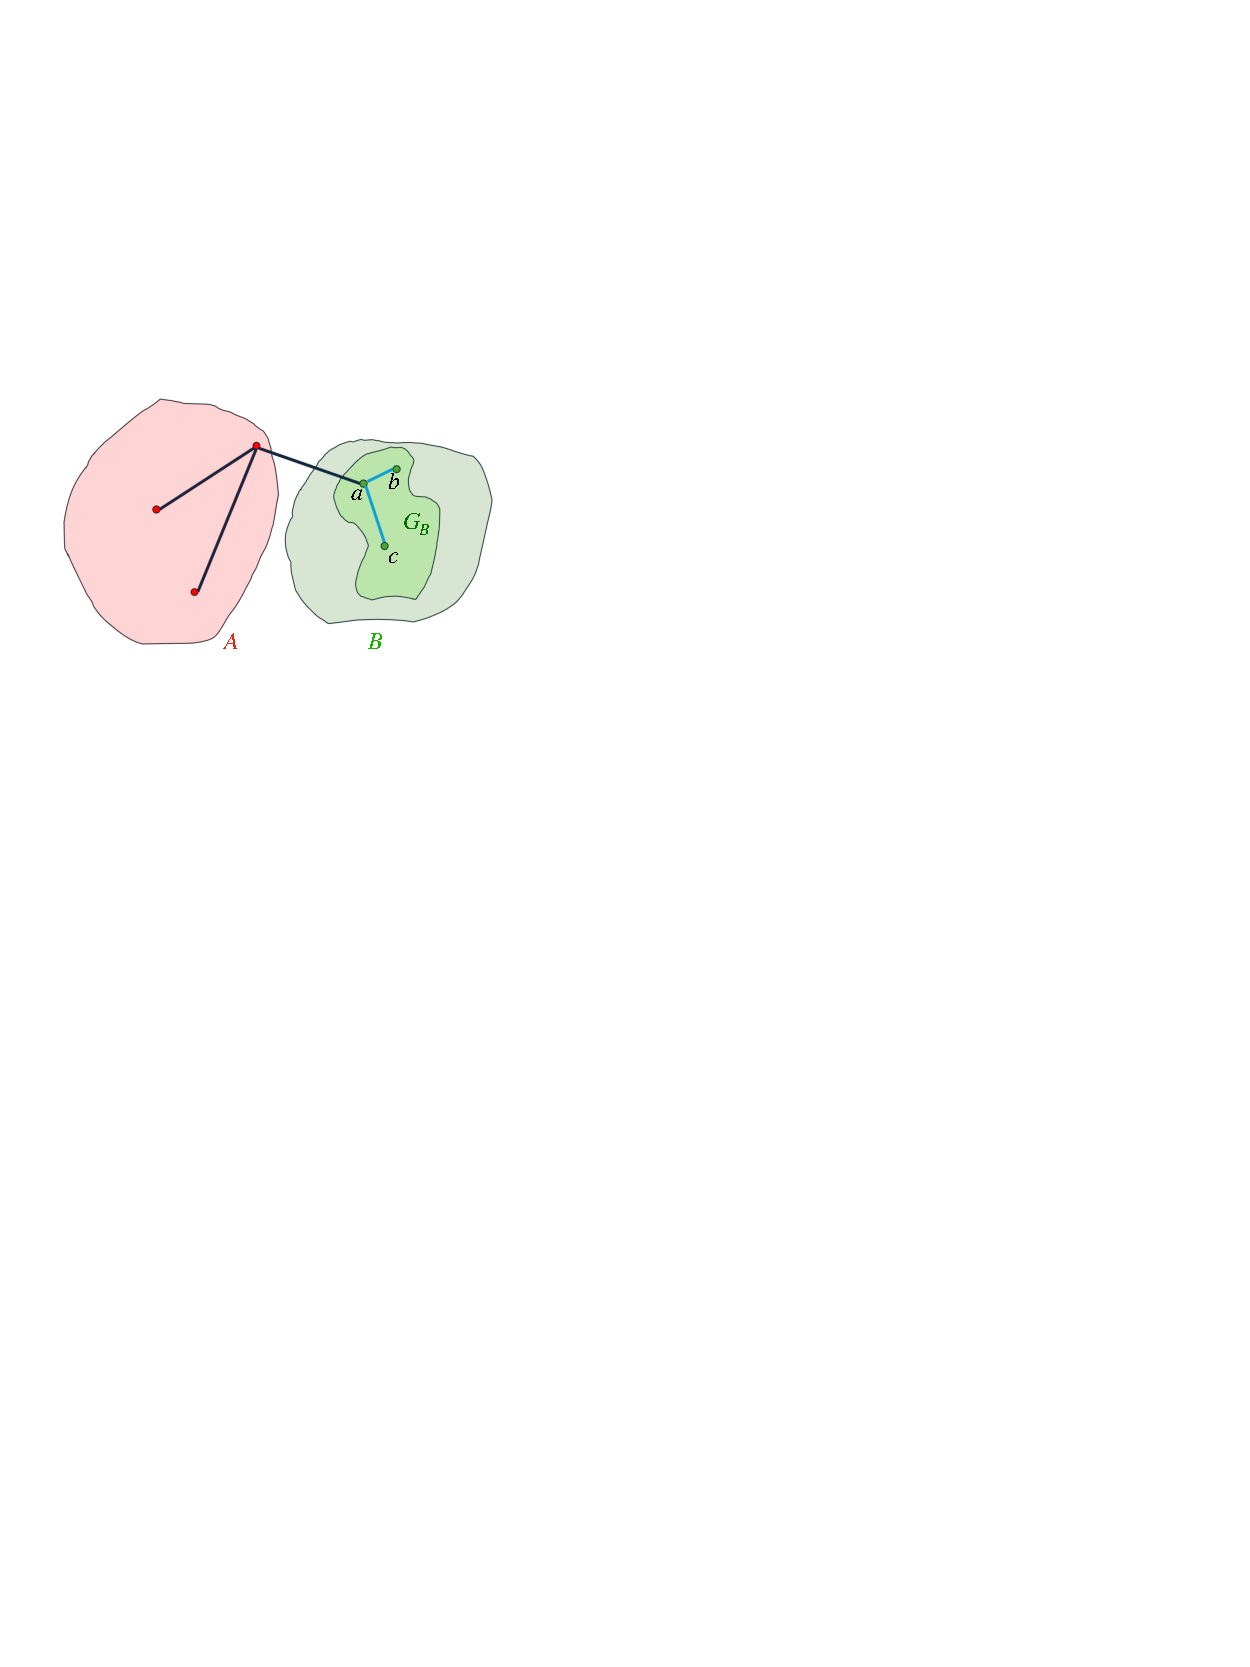
\includegraphics[width=\textwidth]{assets/partition-a.pdf}
%         \caption{}
%       \label{fig:partition}
%     \end{subfigure}%
%     \hspace{1mm}
%     \hspace{1mm}    
%     \begin{subfigure}[t]{0.45\textwidth}
%         \centering
%         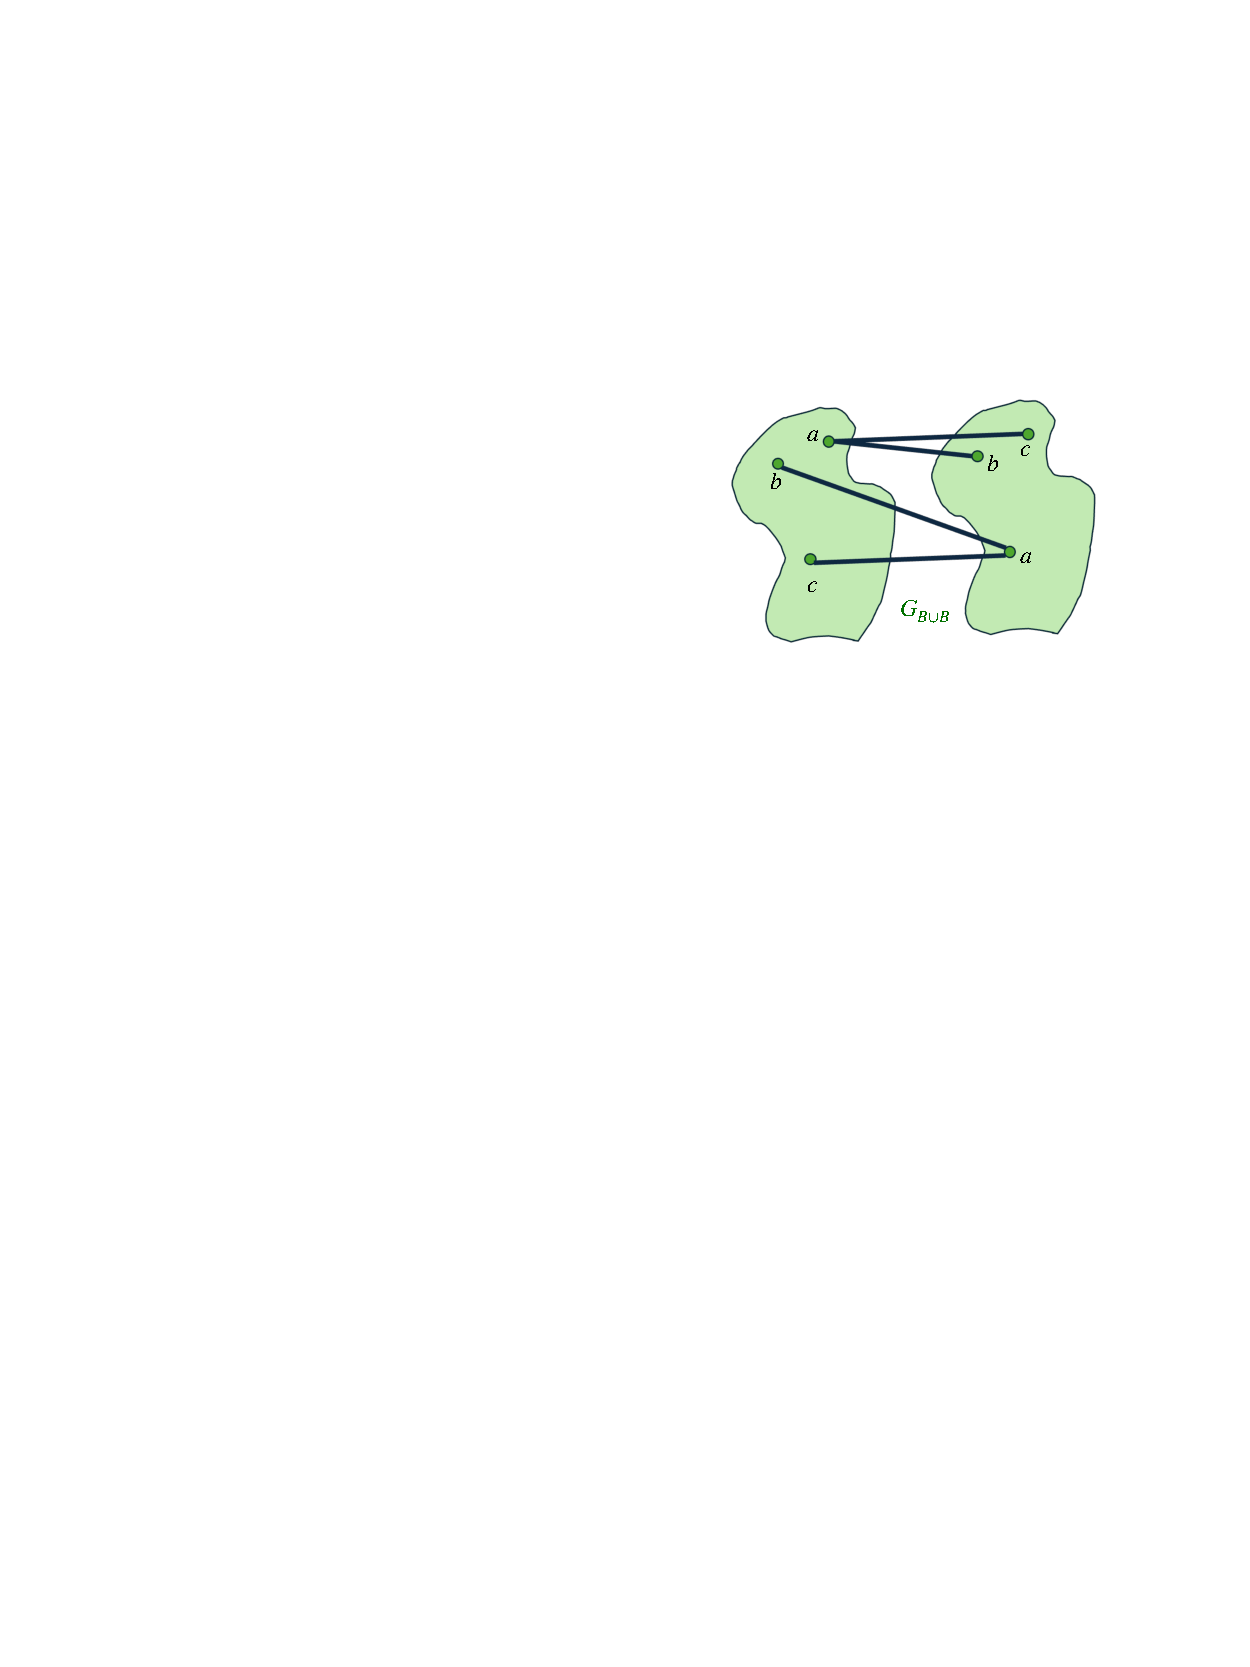
\includegraphics[width=\textwidth]{assets/partition-b.pdf}
%         \caption{}
%       \label{fig:bipartite}        
%     \end{subfigure}
%     \caption{\small The figure above describes the partitioning of the vertices of the graph $G$ into two sets $\RedA$ and $\GreenB$, such that for every vertex $v \in \Vertices{G}$ has at least $11d/16$ \red{red} neighbours and at most $13d/16$ \red{red} neighbours. The subgraph $G_{\GreenB}$ obtained by including vertices in $\GreenB$ and edges that stay inside $\GreenB$. The figure on the right, depicts how the subgraph $G_{\GreenB}$ can be expressed as a bipartite graph $\BipartiteG$.}
%     \hspace{1mm}     
% \end{figure*}


\begin{definition}[Balanced Cuts]\label{defn:balanced-cuts} Given universal constants $0 \leq c \leq 1$ and $\epsilon > 0$, a $(c, \epsilon)$-degree balanced cut of a graph $G$ is a partition $\RedA \cup \GreenB$ of the vertices of $G$, such that, for every vertex $u \in \Vertices{G}$,  $cd - \epsilon d \leq \Neighbourhood{E}{u} \cap \RedA \leq cd + \epsilon d $    
\end{definition}


\begin{lemma}[Regular Graphs Have Balanced Cuts]\label{thm:partition}
For every $0 < c < 1$, and $\epsilon > 0$, there exists a constant $d_0 \in \BigOTilde{c/\epsilon^2}$, such that, given a $d$-regular graph $\Graph = (V, E)$ on $n$ vertices, with $d \in [d_0, n-1]$, there exists and a  sets $\red{A}$ and $\green{B}$ is a $(c, \epsilon)$ balanced cut of $G$.
\end{lemma}

\begin{proof}
  We prove the existence of such a partition $\RedA \cup \GreenB = V$ using the probabilistic method.
We refer to elements in $\RedA$ as red nodes, and elements in $\GreenB$ as green nodes.
For each $v \in \Vertices{\Graph}$, we toss an independent coin $X_i$ with bias $c$.
If $X_i = 1$, then we include $v$ in $\RedA$, else we put $v$ in $\GreenB$.
Thus, $\vec{X} \Def (X_1, \dots, X_n) \in \bit^n$ is a random variable that describes how we partition $V$ into sets $\RedA$ and $\GreenB$.
For any $v \in V$, let $Y_v \Def |\Neighbourhood{E}{v} \cap \RedA|$ denote the random variable that counts how many \red{red} neighbours of $v$ has.
Define $\delta \Def \frac{\epsilon}{c}$, and for any $v \in V$, let $E_v = \Indicator{|Y_v - d c | \geq \delta c d}$ denote the bad event that $v$ has too many \red{red} neighbours.
Observe that the dependency graph of events $\{ E_v \}_{v \in V}$ has max-degree at most $d^2$ (only vertices at most two hops away from $v$ affect the colours of $v$'s neighbours; there at most $d^2$ such vertices).
% To see why, for any node $v$, let $u$ and $w$ denote vertices exactly 2 hops\footnote{A node $a$ is $k$ hops away from another node $b$ if the shortest path between $a$ and $b$ has $k$ edges.} and at least 3 hops away from $v$ respectively. The colour of $u$'s neighbours, directly affects how many red neighbours $v$ can have.
% However, as the colours for each node is sampled independently, the colour of $w$ or its neighbours do not affect $v$'s neighbours.
% Therefore $E_v$ is independent of $E_w$.
% There are at most $d^2$ nodes at a distance of at most 2 from any node, giving us the max-degree of the dependency graph.
As $\Graph$ is $d$-regular, $\Mean{\vec{X}}{Y_v} = c d$, then by the \nameref{lemma:mult-chernoff}, for any $v \in V$, we have $\PProb{E_v}{\vec{X}} \leq 2\exp(-\delta^2c d/3) \Def \beta$.
For $d_0 \in \BigOTilde{c/\epsilon^2}$, we have for every $d > d_0$,  $2\exp(-\delta^2c d/3) \leq 1/(4d^2)$.
Therefore, we have $\beta d^2 \leq 1/4$.
We have all the conditions to invoke the \nameref{lemma:lll} to get $\PProb{\underset{{v\in V}}{\land}\Complement{E_v}}{\vec{X}} > 0$.
\end{proof}


%We are given a pseudorandom graph $G$ on an odd number of vertices for $n$ large enough, and we want to show that refuting perfect matchings in the PC and SoS proof system requires large proofs.
%As described earlier, we do this by topologically embedding the above hard instance $H$ into $G$ while preserving the hardness of the original instance.

% \begin{remark}
%   \label{remark:edge-dist}
% For this section, and the next, we invoke Lemma \ref{thm:partition} with parameters. $c=3/4$ and $\epsilon=1/16$.
% Reviewing the properties of a balanced sets with $c=3/4$ and $\epsilon=1/16$, we have that every vertex $u$ in any $\EnDeeLambda$ graph  $G=(V,E)$,

  
% \end{remark}

\begin{theorem} \label{thm:perfect-matching}
Suppose $G$ is an $(n, d, \lambda)$-graph, where $\lambda < d/50$. If $U \subseteq V(G)$ is of even size and $\delta(G[U]) \ge 11d/16$, then $G[U]$ contains a perfect matching.
\end{theorem}
\begin{proof}
  Suppose $U \subseteq V(G)$ is of even size and $\delta(G[U]) \ge 11d/16$.
  We show that $G[U]$ satisfies a stronger version of Tutte's criterion:  $S \subseteq U$, $G[U \setminus S]$ has at most $|S|$ connected components.
  If $|S| \ge |U|/2$ then the criterion trivially holds, thus we can assume $|S| < |U|/2$.
  It suffices to show that for every partition $X \cup Y$ of $U \setminus S$ such that $|X|, |Y| \ge |S|/3$, there exists an edge between $X$ and $Y$.
  Indeed, suppose that this holds but $G[U \setminus S]$ has more than $|S|$ connected components, with vertex sets denoted by $C_1, \ldots, C_k$, for some $k > |S|$.
  Then there is no edge between $X := C_1 \cup \ldots \cup C_{s}$ and $Y := C_{s+1} \cup \ldots \cup C_{k}$, where $s = \lfloor |S|/2 \rfloor \ge |S|/3$. As $|X|, |Y| \ge |S|/3$, we get a contradiction. 

    Consider some partition $X \cup Y$ of $U \setminus S$ with $|X| \le |Y|$. Then $|X| \le (|U| - |S|)/2 \le (n - |S|)/2$. We show
    \begin{equation} \label{eq:edge_bound}
        e(X, X) + e(X, S) < \frac{11d}{16}|X|,
    \end{equation}
    as then the minimum degree assumption on $G[U]$ implies there has to be an edge with one endpoint in $X$ and the other in $U \setminus (X \cup S) = Y$. By the Expander Mixing Lemma we have
    \[
        e(X, X) + e(X, S) \le \frac{d}{n}|X|^2 + \lambda |X| + \frac{d}{n}|X||S| + \lambda\sqrt{|X||S|}.
    \]
    Using $|S|/3 \le |X| \le (n-|S|)/2$, $|S| \le n/2$, and $\lambda < d/24$,  we further upper bound the right hand side:
    \[
        \frac{d}{n} |X| \frac{n-|S|}{2} + \lambda |X| + \frac{d}{n}|X||S| + \lambda\sqrt{3} |X| < \frac{d}{2}|X| + \frac{d}{n}|X||S| + 3 \lambda |X| \le \frac{d}{4} |X| + 3\lambda |X| < \frac{11d}{16}|X|.
    \]
    This confirms \eqref{eq:edge_bound}.
\end{proof}

\section{Embedding Machinery}
\label{sec:embed-machinery}

The following definitions are adapted from \citep{nenadov2023routing} but were originally introduced by \citet{feldman1988wide} in their work about the theory of wide sense blocking networks.

\begin{definition}[$(p, q)$-non blocking bipartite graphs]
Given $p,q \in \Naturals$, we say that a bipartite graph $\Graph = (A \cup B, E)$ is $(p, q)$ \emph{non-blocking}, if there exists a collection  $\Family{S}$ of subsets of $E$, called the \emph{safe states}, such that the following holds:

\begin{enumerate}
	\item $\emptyset \in \Family{S}$
	\item If $E'' \subseteq E'$ and $E' \in \Family{S}$, \emph{then}, $E'' \in \Family{S}$.
	\item Given $E' \in \Family{S}$ such that $|E'| \leq q$, and \emph{any} $v \in A$ with $\degree{E'}{v} < p$, there exists $e = (v, w) \in E \setminus E'$  such that (i) $E' \cup \Set{e} \in \SafeStates $, and (ii) $w$ is not incident to any edge in $E'$ i.e. $\forall x \in A$ we have $(x,w) \notin E'$. 
 We call $w$ a \emph{safe neighbour} for $v$ given $E'$.
\end{enumerate}

\end{definition}


% \begin{figure}[h]
%   \center
%   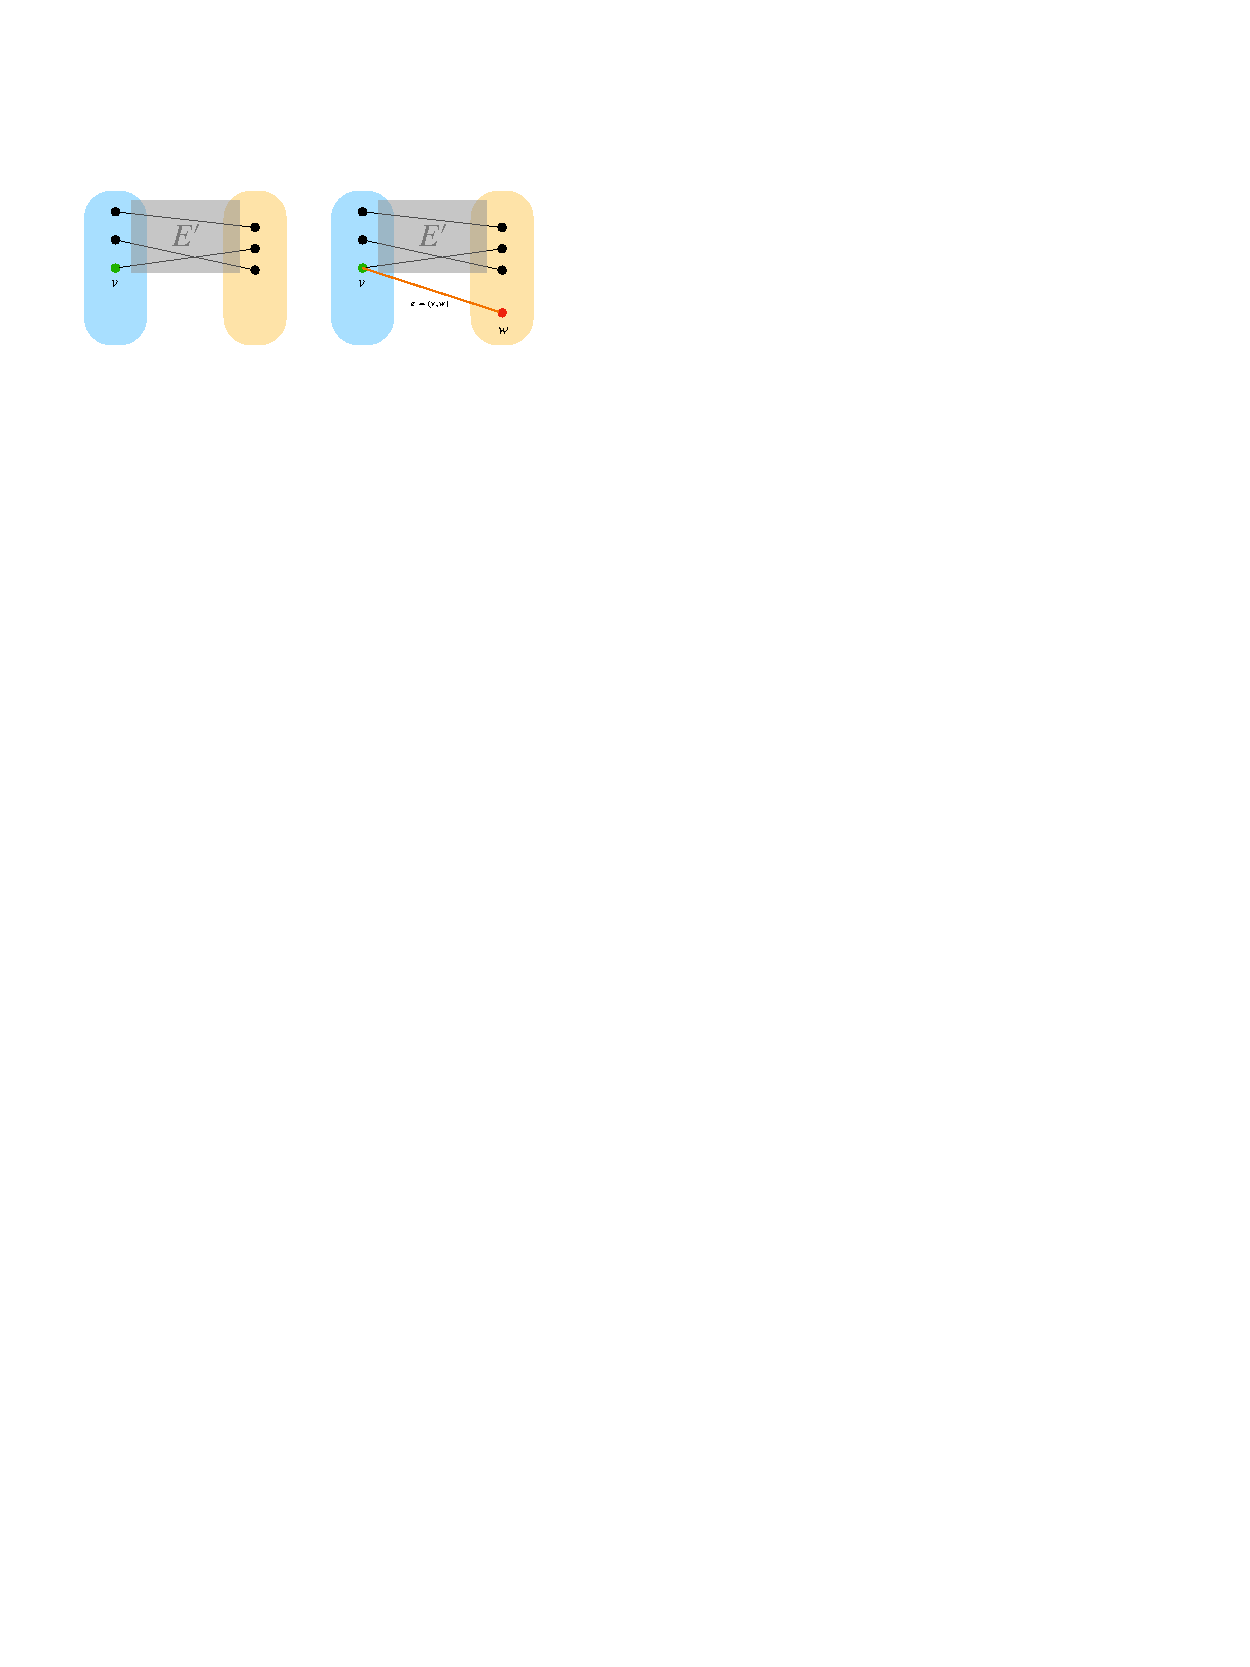
\includegraphics{assets/non-blocking-networks.pdf}
%   \caption{\small The figure above demonstrates the third property of non blocking bipartite graphs $G=(L\cup R, E)$.
%       Assume $E' \subseteq E$ is a safe state with size less than $q$ and that $v$ has fewer than $p$ neighbours in $E'$.
%       Then by the non blocking property, we are \emph{guaranteed} to connect $v$ to a safe neighbour $w \in R$ that has no incident edges from $E'$.}
% \label{fig:test}
% \end{figure}

Next, we re-state a lemma by \citep[Proposition 1]{feldman1988wide} which describes the properties bipartite graphs must satisfy to be non-blocking.

\begin{lemma}\label{lemma:condtions-for-non-block}
Fix $a, r, s \in \Naturals$. Let $\Graph = (X \cup Y, E)$ be a bipartite graph.
If for every $S \subseteq Y$ of size $1 \leq |S| \leq 2a$, there are \emph{at least} $(r + s)|S|$ neighbours in $Y$ that are adjacent to $S$, \emph{then}, $\Graph$ is $(r, as)$-non blocking.
\end{lemma}

The above definition and lemma are all we need to describe our embedding machinery.

\begin{lemma}\label{lemma:bipartitie-is-non-blocking}Let $G$ be the $\EnDeeLambda$ graph with $\lambda \leq d/50$. For any $\GreenB \subseteq \Vertices{G}$ such that $\MinimalDegree{G[\GreenB]} \geq \nicefrac{3d}{16}$,
 the bipartite graph  $\BipartiteG = (G[\GreenB] \cup G[\GreenB], \Edges{G[\GreenB]})$ is $(\frac{d}{\lambda},  n/20)$ non-blocking.
\end{lemma}

\begin{proof}
  Define $c_1 = 20$ and $c_2 = 50$. Let $X$ and $Y$ denote the right vertices of $\BipartiteG$.
  Set $a = \frac{n\lambda}{2c_1 d}$.
  Observe that that $\left(\frac{1}{c_1/2}  + \sqrt{\frac{1}{c_2/2}}\right) < \frac{3}{16}$.
Let $S \subseteq X$ with $|S| \leq 2a = \frac{n\lambda}{c_1 d}$.
\highlight{Assume towards a contradiction} that $\BipartiteG$ is \textbf{not} non-blocking.
  Then by Lemma \ref{lemma:condtions-for-non-block} there exists a set $T \subseteq Y$, adjacent to vertices in $S$ such that $|T| < |S|(\frac{d}{\lambda}+\frac{d}{\lambda})$. 
As $G[\GreenB]$ has minimal degree at leat $\nicefrac{3d}{16}$, 

\begin{equation}\label{eq:balanced}
  \CutEdges{S}{T}{E_{\GreenB}} \geq \frac{3}{16}|S|d
\end{equation}

However, $S$ and $T$ are also subsets of $\Vertices{G}$ and $G$ is a $\EnDeeLambda$ graph.
From the \nameref{lemma:expanders-mixing-lemma}, we have

\begin{align}
  \CutEdges{S}{T}{E_{\GreenB}} &\leq   \CutEdges{S}{T}{E} \\
  &\leq \frac{d}{n}|S||T| + \lambda\sqrt{|S||T|} \\
	&< 2\frac{2d^2}{n\lambda}|S|^2 + |S|\sqrt{2\lambda d} \label{eq:assumption}\\
	&\leq |S|\left(\frac{2d^2}{\lambda n} \frac{n\lambda}{c_1 d} + \sqrt{d\cdot \frac{d}{c_2/2}}\right) \label{eq:assumption-lambda}\\
	&= |S|d\left(\frac{1}{c_1/2}  + \sqrt{\frac{1}{c_2/2}}\right) \\
	&< |S|d\frac{3}{16} \label{eq:constants}
\end{align}

\eqref{eq:assumption} comes from our \highlight{assumption} on the size of $T$..
\eqref{eq:assumption-lambda} comes from our assumption that $\lambda \leq  d/c_2$ and $|S| \leq \frac{n\lambda}{c_1 d}$.
\eqref{eq:constants} contradicts the balanced sets property in Equation \eqref{eq:balanced}, so our \highlight{assumption} must have been wrong.
Therefore $\BipartiteG$ is $(\frac{d}{\lambda}, \epsilonA n)$ non blocking.
\end{proof}


\begin{definition}[Sub-divisions]\label{def:subdivisions}
Given a graph $H$ and a function $\sigma: \Edges{H} \rightarrow \Naturals$, the $\sigma$-subdivision of $H$, denoted by $\Subdivision{H}{\sigma}$, is the graph obtained by replacing each edge in $\Edges{H}$ with a path of length $\sigma(e)$ joining the end points of $e$ such that all these paths are mutually vertex disjoint, except at the end points.	
\end{definition}

\begin{definition}[Topological Minor]\label{def:topological-minor}
A graph $H$ is a topological minor of a graph $G$ if there exists a subdivision $\Subdivision{H}{\sigma}$ that is isomorphic to \emph{any} subgraph of $G$.	
\end{definition}


\begin{theorem}[Embedding Theorem]\label{theorem:embedding-theorem}
  Let $G=(V,E)$ denote an $\EnDeeLambda$ graph with $\lambda \le d/50$, and $H$ be an arbitrary sparse graph with at most $t = \lfloor \frac{ n}{20\MaxDegree{H}\log_Dn}\rfloor $ vertices with max degree $\MaxDegree{H} = \BigO{1} < d$, where $D=d/\lambda$.
  For any subset $\GreenB \subseteq V$ of size $\Size{\GreenB} \ge \frac{3n}{16}$ and $\MinimalDegree{G[\GreenB]} \ge \frac{3d}{16}$, $G[\GreenB]$ contains $H$ as a topological minor $\Subdivision{H}{\sigma}$ where every edge in $H$ is an odd sized path in $\Subdivision{H}{\sigma}$.
\end{theorem}

\begin{proof}
Let $D = \frac{d}{\lambda}$ and $k =  \lceil\log_D n\rceil$.
Let $\{ h_1, \dots, h_t\}$ denote the vertices of $H$.
Define $\sigma(e) \Def 2k+1$ for all $e \in \Edges{H}$.
Let $\EmbeddingFunc: \Vertices{\Subdivision{H}{\sigma}} \rightarrow \Vertices{G[{\GreenB}]}$ be the bijective mapping which will be our toplogical embedding.
Our first task is to find a unique $\Embedding{h} \in \Vertices{G[\GreenB]}$ for each $h \in \Vertices{H}$.
Define $X = Y = \Vertices{G[\GreenB]}$, and let $\BipartiteG = (X \cup Y, \Edges{G[\GreenB]})$.
Let $\{a_1, \dots, a_{t}\}$ be arbitrary set of $t$ vertices in $G[\GreenB]$.
As $\MinimalDegree{G[\GreenB]} \geq \nicefrac{3d}{16}$, by Lemma \ref{lemma:bipartitie-is-non-blocking} we know have that $\BipartiteG$ is $(D, n/20)$ non-blocking.
We repeat the following process to obtain $\{ \Embedding{h_1}, \dots, \Embedding{h_t}\}$: 

\begin{itemize}
\item Define $E' = \emptyset$ which is guaranteed to be a  safe state.
  
\item For $a_1 \in X$, we ask for $D$ neighbours in $Y$. As $E'$ is a safe state, we can always find at least one safe neighbour $\tilde{h}_1 \in Y$. We set $\Embedding{h_1} \Def \tilde{h}_1$ and update $E' = E'  \cup \{(a_1, \tilde{h}_1)\}$.
  
\item We repeat this process for all $a \in \{a_2, \dots, a_t\}$. For the $j$'th step, As $|E'| = j \leq t < n/20$, for each $a_j$ we can always find a safe neighbour $\Embedding{h_j} \in Y$.
  
\end{itemize}

Once this phase is complete, we have mapped every vertex of $H$ to a unique vertex in $G[\GreenB]$.
The next step to show that for each $(u,v) \in \Edges{H}$, there is a vertex disjoint path of length $2k+1$ between $\Embedding{u}$ and $\Embedding{v}$ in $G[\GreenB]$.
Let $(e_1, \dots, e_m)$ be an arbitrary ordering of edges in $\Edges{H}$.
We prove the result by induction on $m$. Define a global edge set  $\GlobalEdgeSet \Def \emptyset$.

\paragraph{Base case} 

Let $e_1 = (u_1,v_1)$. Define sets $S_0 = \{\Embedding{u_1}\}$ and $S'_0 = \{ \Embedding{v_1}\}$, and set $M_0 = \emptyset$ and $M_0' = \emptyset$.
We will define edge sets $\{ M_j\}_{j \in [k]}$ and $ \{ M'_j\}_{j \in [k]}$, and vertex sets $\{ S_j\}_{j \in [k]}$ and $\{ S'_j\}_{j \in [k]}$ inductively as follows: For each $1 \leq j \leq k$, we construct $S_{j}$ with the following process.
For each $x \in S_{j-1}$, find the corresponding copy $x \in X$. Ask for $D$ neighbours of $x$ in $Y$ via edges in $\Edges{\BipartiteG}$.
With respect to $\GlobalEdgeSet \cup \Big(\cup_{i=1}^{j} (M_i \cup M'_i)\Big)$, add $\Size{M_j}$ safe neighbours to $S_{j+1}$ where $\Size{M_j} \le \min\{t, |S_{j-1}|D\}$.
Add to $M_j$ the safe edges that connect $S_{j-1}$ to $S_j$.
$M_j'$ and $S_j'$ are defined analogously.
Note that for $1 \le j \le k$, as there at most $t$ edges in each $M_j$, there are a total of $2tk < n/20$ edges in $\cup_{i=1}^{k} (M_i \cup M'_i)$.
Thus, we can always find at least $t$ safe edges been $ S_{j-1}$ and $S_j$ for every $1 \le j \le t$.
Now as $k = \log_D[n]$, we have that, $|S_k| = |S_k'|= t$.
By the expander mixing lemma \ref{lemma:expanders-mixing-lemma},

\begin{align}
\CutEdges{S_k}{S_k'}{E}
 &\geq \frac{d t^2}{n} - \lambda t  > 0 \label{eq:assumption_on_lambda}
\end{align}

Equation \eqref{eq:assumption_on_lambda} comes from the assumption $\lambda \leq d/50$.
This implies there exists at least one edge $e^\star=(x^\star,y^\star) \in \CutEdgesSet{S_k}{S_k'}{\Edges{\BipartiteG}}$.
By how we constructed $M_k$, we know that $x^\star$ was the safe neighbour of some node $a \in S_{k-1}$.
Let $m_k = (a,x^\star) \in M_k$ be the connecting edge.
Similarly, there is some edge $m_{k-1} \in M_{k-1}$ that connects some vertex in $S_{k-2}$ to $a$ with a safe edge.
We repeat this process all the way, till we get $k+1$ edges, $m_1 m_2 \dots, m_k, e^\star$.
We repeat the same process for the other end point of $y \in S_k'$, to get edges $e^\star, m'_1, \dots, m'_k$.
We add these edges to a global edge set $\GlobalEdgeSet$.
Thus, we have found an odd length path $m_1\dots m_k e^\star m_1'\dots m_k'$ of length $2k+1$, connecting $\Embedding{u}$ to $\Embedding{v}$.
 % Figure \ref{fig:baseB} illustrates everything discussed so far pictorially.


\paragraph{Induction Step}
	
Assume that we have found paths for $e_1 = (u_1, v_1), \dots, e_j=(u_j, v_j)$ for $j < m$.
Let $P_1, \dots, P_j$ denote these paths.
$\GlobalEdgeSet$ denotes this set of all edges in these paths.
We upper bound the size of $\GlobalEdgeSet$.
$H$ has at most $\frac{t\MaxDegree{H}}{2}$ edges.
When these edges are mapped to paths of length $2k+1$, the total number of edges is $\frac{t\MaxDegree{H}}{2}(2k+1) <  \frac{n}{10\MaxDegree{H}}$.
Thus not only is $\GlobalEdgeSet$ strictly smaller than $n/20$ but it has room for $2tk+1$ more edges with room to spare i.e. $\frac{n}{10\MaxDegree{H}}+ 2tk + 1 < n/20$.
Now we once again do what we did in the base case.
We set $S_0 = \{ u_{j+1}\}$ and $S_0' = \{v_{j+1} \}$.
For all $1 \le j \le k$, we set $S_{j}$ to be $\min\{t, \Size{S_{j-1}}D \}$ safe neighbours adjacent to $S_{j-1}$.
Now finding a path for $e_{j+1} = (u_{j+1},v_{j+1}) \in \Edges{H}$ reduces to the base case.
This concludes the proof.
	
\end{proof}

\section{Proof Of Main Result}
\label{sec:main-proof}

Let $G=(V,E)$ denote any $\EnDeeLambda$-graph on an odd number of vertices, and,  $\HardInstance$ denote the hard instance on $t=\BigO{\frac{n}{\log n}}$ vertices for which refuting $\PM{H}$ has degree $\BigOmega{t}$ as per Lemma \ref{lemma:worst-case-instance-sos}.
Then hardness proof for refuting $\PM{G}$ follows from the following steps as illustrated in Figure \ref{fig:proof-outline}.


\begin{enumerate}
\item{Invoke Theorem \ref{thm:partition} with parameters $c=3/4$ and $\epsilon = 1/16$ to get a partition of $V = \RedA \cup \GreenB$ such that for every $u \in V$: $\frac{11}{16}d  \leq   \Size{\Neighbourhood{E}{u} \cap \RedA} \leq \frac{13}{16}d$ and $\frac{3}{16}d  \leq   \Size{\Neighbourhood{E}{u} \cap \GreenB} \leq \frac{5}{16}d$.}
  
\item{As $\MinimalDegree{G[\GreenB]} \geq \frac{3d}{16}$, and $\MaxDegree{H} = 5 < d$,and $\lambda < \epsilonL d$, we can invoke Theorem \ref{theorem:embedding-theorem} to embed $H$ as a topological minor $G_{\EmbeddingFunc}$ in $G[\GreenB]$ such that every edge $(u,v)$ in $H$ is an odd length path $\Path{\Embedding{u}}{\Embedding{v}}$ in $G_{\EmbeddingFunc}$.
    Then it is at least as hard to refute\footnote{Note that this by itself does not guarantee it is hard to refute $\PM{G}$. We need item (3) and this to show hardness in refuting $\PM{G}$.} $\PM{G_{\EmbeddingFunc}}$ as it is to refute $\PM{H}$.    
    To see why, map each variable $y_e$ for $e \in \Path{\Embedding{u}}{\Embedding{v}}$ alternately to $x_{uv}$ or $\bar{x}_{uv}$, such that the edges adjacent to $\Embedding{u}$ and $\Embedding{v}$ are set to $x_{uv}$. This is always possible as $\Path{u}{v}$ is off odd length. Observe that this function maps a perfect matching formula  $\PM{G_{\EmbeddingFunc}}$ to $\PM{H}$. Therefore it should be at least as hard to refute $\PM{G_{\EmbeddingFunc}}$ as it is to refute $\PM{H}$.
  }

\item{ As $n$ is odd, and $\Size{\Vertices{G_{\EmbeddingFunc}}}$ is odd, we have that $U = V \setminus G_{\EmbeddingFunc}$ has even size.
    The balanced partitioning gives us $\MinimalDegree{G[U]} \geq \frac{11d}{16}$, and as $\lambda \leq d/50 < ?$, we can inoke Theorem \ref{thm:perfect-matching} to show $G[U]$ has a perfect matching $M$.
Define map $\rho: \{x_1, \dots, x_{|\Edges{G}|}\} \rightarrow \{x_1, \dots, x_{|\Edges{G}|}, \bar{x}_1, \dots, \bar{x}_{|\Edges{G}|}, 1, 0 \}$ such that 
	

\[
\rho(x_e) =
\left\{
\begin{array}{@{}cl}
x_e & \text{if } e \in \Edges{G_{\EmbeddingFunc}} \\
1 & \text{if } e \in M \\
0 & \text{otherwise}
\end{array}
\right.
\]

	If it easy to see that $\PM{G} \equiv \PM{G}|_\rho \equiv \PM{H}$. Therefore by Lemma \ref{lemma:affine_restriction} above, we get that $\PM{G} \in \BigOmega{|\Vertices{H}|} = \BigOmega{\frac{n}{\log n}}$. }
  \end{enumerate}


\section{Related Work}
\label{sec:related-work}


\bibliographystyle{unsrtnat}
\bibliography{perfect-matchings-main}
\clearpage
\appendix



\end{document}
